% This is samplepaper.tex, a sample chapter demonstrating the
% LLNCS macro package for Springer Computer Science proceedings;
% Version 2.20 of 2017/10/04
%
\documentclass[runningheads]{llncs}
%
\usepackage{graphicx}
\usepackage{listings}
\usepackage{microtype}                 % use micro-typography (slightly more compact, better to read)
\PassOptionsToPackage{warn}{textcomp}  % to address font issues with \textrightarrow
\usepackage{textcomp}                  % use better special symbols
\usepackage{mathptmx}                  % use matching math font
\usepackage{times}                     % we use Times as the main font
\usepackage{enumitem}
\renewcommand*\ttdefault{txtt}         % a nicer typewriter font
%\usepackage{cite}                      % needed to automatically sort the references
\usepackage{tabu}                      % only used for the table example
\usepackage{booktabs}                  % only used for the table example
\usepackage{amsmath,amssymb,amsfonts}
\usepackage{subcaption}
\usepackage{framed}
\usepackage{lineno,hyperref}
\newcommand{\fix}[1]{\textcolor{red}{\textbf{\textit{#1}}}}
\newcolumntype{P}[1]{>{\centering\arraybackslash}p{#1}}
\newcolumntype{L}[1]{>{\raggedleft\arraybackslash}p{#1}}
\usepackage[dvipsnames]{xcolor,colortbl}
\newcommand{\mc}[2]{\multicolumn{#1}{c}{#2}}
\definecolor{Gray}{gray}{0.85}
\definecolor{LightCyan}{rgb}{0.88,1,1}
\definecolor{LightRed}{rgb}{1,0.88,1}

\newcolumntype{a}{>{\columncolor{Gray}}c}
\newcolumntype{b}{>{\columncolor{LightCyan}}c}
\newcolumntype{d}{>{\columncolor{LightRed}}c}

\usepackage[subrefformat=parens,labelformat=parens]{subcaption}
\usepackage{multirow}
\usepackage{tikz}
\usepackage{collcell}

\newenvironment{tightEnumerate}{
\begin{enumerate}
        \setlength{\itemsep}{1pt}
        \setlength{\parskip}{0pt}
        \setlength{\parsep}{0pt}
}{\end{enumerate}
}

\newenvironment{tightItemize}{
\begin{itemize}
        \setlength{\itemsep}{1pt}
        \setlength{\parskip}{0pt}
        \setlength{\parsep}{0pt}
}{\end{itemize}
}


\newcommand*{\MinNumberR}{0.0}%
\newcommand*{\MaxNumberR}{20}
\newcommand{\ApplyGradientR}[1]{%
        \pgfmathsetmacro{\PercentColor}{100.0*(#1-\MinNumberR)/(\MaxNumberR-\MinNumberR)}
        \hspace{-0.33em}\colorbox{red!\PercentColor!white}{#1}
}

\newcolumntype{R}{>{\collectcell\ApplyGradientR}c<{\endcollectcell}}



\newcommand*{\MinNumberD}{0}%
\newcommand*{\MaxNumberD}{100}
\newcommand{\ApplyGradientD}[1]{%
        \pgfmathsetmacro{\PercentColor}{100.0*(#1-\MinNumberD)/(\MaxNumberD-\MinNumberD)}
        \hspace{-0.33em}\colorbox{red!\PercentColor!white}{#1}
}







\newcolumntype{D}{>{\collectcell\ApplyGradientD}c<{\endcollectcell}}



\newcommand*{\MinNumberA}{0.0}%
\newcommand*{\MaxNumberA}{0.08}
\newcommand{\ApplyGradientA}[1]{%
        \pgfmathsetmacro{\PercentColor}{100.0*(#1-\MinNumberA)/(\MaxNumberA-\MinNumberA)}
        \hspace{-0.2em}\vspace{-0.05em}\colorbox{orange!\PercentColor!white}{#1}
}

\newcolumntype{A}{>{\collectcell\ApplyGradientA}c<{\endcollectcell}}


\newcommand*{\MinNumberB}{0.0}%
\newcommand*{\MaxNumberB}{10.0}
\newcommand{\ApplyGradientB}[1]{%
        \pgfmathsetmacro{\PercentColor}{100.0*(#1-\MinNumberB)/(\MaxNumberB-\MinNumberB)}
        \hspace{-0.2em}\colorbox{orange!\PercentColor!white}{#1}
}

\newcolumntype{B}{>{\collectcell\ApplyGradientB}c<{\endcollectcell}}


\newcommand*{\MinNumberC}{0.0}%
\newcommand*{\MaxNumberC}{0.44}
\newcommand{\ApplyGradientC}[1]{%
        \pgfmathsetmacro{\PercentColor}{100.0*(#1-\MinNumberC)/(\MaxNumberC-\MinNumberC)}
        \hspace{-0.2em}\colorbox{orange!\PercentColor!white}{#1}
}

\newcolumntype{C}{>{\collectcell\ApplyGradientC}c<{\endcollectcell}}


\newcommand*{\MinNumberN}{0.0}%
\newcommand*{\MaxNumberN}{0.75}
\newcommand{\ApplyGradientN}[1]{%
        \pgfmathsetmacro{\PercentColor}{100.0*(#1-\MinNumberN)/(\MaxNumberN-\MinNumberN)}
        \hspace{-0.33em}\colorbox{red!\PercentColor!white}{#1}
}

\newcolumntype{N}{>{\collectcell\ApplyGradientN}c<{\endcollectcell}}

\usepackage{epstopdf}
\epstopdfsetup{outdir=./}
% Used for displaying a sample figure. If possible, figure files should
% be included in EPS format.
%
% If you use the hyperref package, please uncomment the following line
% to display URLs in blue roman font according to Springer's eBook style:
% \renewcommand\UrlFont{\color{blue}\rmfamily}

\begin{document}
%
\title{Investigating the Use of In Situ Reduction \\via Lagrangian Representations for \\Cosmology and Seismology Applications}
%
\titlerunning{Lagrangian Representations for Cosmology and Seismology Applications}
% If the paper title is too long for the running head, you can set
% an abbreviated paper title here
%
%\author{Sudhanshu Sane\inst{1}\orcidID{0000-1111-2222-3333} \and Hank Childs\inst{2}\orcidID{1111-2222-3333-4444}}
%
%\authorrunning{S. Sane et al.}
% First names are abbreviated in the running head.
% If there are more than two authors, 'et al.' is used.
%
%\institute{SCI Institute at University of Utah, USA \and University of Oregon, USA}
%
\maketitle              % typeset the header of the contribution
%
\begin{abstract}
%Although a large number of applications produce time-varying vector fields, many limit subsequent analysis to single time slices due to constraints on data storage.
%%
%In recent years, reduced Lagrangian representations of time-varying vector fields have been researched as a potential approach to enable accurate post hoc analysis.
%%
%The utility of this technique, however, varies based on the nature of the vector field, and the configuration specifics that determine computation costs as well as storage requirements.
%%In recent years, reduced Lagrangian representations of time-varying vector fields have been considered to enable accurate post hoc analysis.
%%
%This paper contributes the investigation of Lagrangian representations computed in situ for two application domains: cosmology and seismology.
%%
%%These applications generate time-varying vector fields that vary in nature to those previously studied.
%%
%To investigate utility, we evaluate effectiveness and viability. 
%%
%To inform effectiveness, our study conducted a statistical analysis of efficacy across a range of spatiotemporal configurations as well as a qualitative evaluation. %comparison of the technique to the traditional Eulerian approach.
%%
%To inform viability, we considered representative HPC environments, integrated in situ infrastructure with the simulation codes, and performed Lagrangian in situ reduction using GPUs as well as CPUs.
%%
%We found that time-varying vector fields produced by the cosmology and seismology applications considered can be reduced by 200X via Lagrangian representations, while maintaining accurate reconstruction and requiring under 10\% of total execution time in 11 of 13 experiments.
%%In particular, we found Lagrangian representations for data generated by the Nyx cosmology simulation are sensitive to both spatial and temporal sampling, notably providing higher accuracy as temporal sparsity increases.
%%
%%For the SW4 seismology simulation, we found Lagrangian representations can accurately encode time-varying vector fields for seismic wave propagation and offer strong data reduction propositions.
%%
%%Additionally, we include results from a benchmarking study using an ECP mini-application that utilizes heterogenous compute resources.
%%
%%Overall, the in situ processing cost to compute Lagrangian representations was under 10\% of total execution time in 11 of 13 experiments.
%%
%
%\fix{HANK:}
Although many types of computational simulations produce time-varying vector fields, 
subsequent analysis is often limited to single time slices due to excessive costs.
%
Fortunately, a new approach using a Lagrangian representation can 
enable time-varying vector field analysis while mitigating these costs.
%
With this approach, a Lagrangian representation is calculated while the simulation code is running, and the result is explored after the simulation.
%
Importantly, 
 the effectiveness of this approach varies based on the nature of the vector field, 
requiring in-depth investigation for each application area.
%
With this study, we evaluate the effectiveness for previously unexplored cosmology and seismology
applications. %, which have previously been unexplored.
%
We do this by considering encumbrance (on the simulation to calculate the
Lagrangian representation) and also efficacy (of the reconstructed result).
%
To inform encumbrance, we 
integrated in situ infrastructure with two simulation codes, 
and evaluated on representative HPC environments,
performing Lagrangian in situ reduction using GPUs as well as CPUs.
%
To inform efficacy, our study conducted a statistical analysis across a range of spatiotemporal configurations as well as a qualitative evaluation.
%
In all, we demonstrate effectiveness for both cosmology and seismology --- time-varying vector fields from these domains can be reduced by 200X via Lagrangian representations, while maintaining accurate reconstruction and requiring under 10\% of total execution time in over 80\% of our experiments.

\keywords{Lagrangian analysis \and in situ processing \and vector data}
\end{abstract}
%
%
%

\section{Introduction}
\label{sec:introduction}
%Top}ics for introduction / related work:
%1. One of the challenges faced by scientists is the data analysis and visualization of the large amounts of data generated by simulation codes on HPC resources.
%2. In situ processing offers a potential solution by circumventing the need to store all the raw data. 
%3. Most in situ analysis tasks operate infrequently or are triggered. Computing Lagrangian flow maps is unlike other analysis tasks and requires computation every cycles of the simulation - this places an overhead on the simulation code and raises questions of viability. 
%4. Lagrangian analysis has been extensively studied for ocean modeling in an offline setting and now efforts to support online analysis are being made.
%5. Reduced Lagrangian flow maps have been shown to be superior to traditional Eulerian subsampling for primarily analytical data sets, in theoretical settings or 2D flows, and compared using a single average error across all post hoc interpolated particles. 
%6. We believe reduced Lagrangian flow maps need to be explored for more real world time-varying vector fields to better understand their applicability, and more closely evalauted - both quantitatively and qualitatively - to understand efficacy characteristics.
%7. We strongly believe Lagrangian flow maps need to be evaluated in representative settings - integrated with a simulation code and executing on a supercomputer - to provide insight into viability.
%8. Given reduced Lagrangian flow maps are a new paradigm - it opens research opportunities along multiple axes - namely, sampling strategy, post hoc interpolation, ease of use (integration), performance (viability) and applicability (configuration settings, vector field type, etc). 
%9. Several works have advanced research along these axes - but none have considered viability in relation to simulation execution times or application to seismology or cosmology vector fields. Demonstration in this form we believe encourages wider adoption of the paradigm beyond the theoretical level.
%
%
%
%
High-performance computing resources play a key role in advancing computational science by enabling modeling of scientific phenomena at high spatiotemporal resolutions.
%
%Although HPC enables modeling of scientific phenomena at high spatiotemporal resolutions, the total data generated is prohibitively large.
%
A challenge with regard to studying the output of a simulation is the prohibitively large size of the total data generated.
%
Compromise in the form of storing a subset of the data can impact the extent and accuracy of subsequent post hoc exploratory analysis and visualization.
%
In particular, for accurate time-varying vector field analysis and visualization, access to the full spatiotemporal resolution is required.
%
Since storing the entire simulation output is expensive, scientists resort to temporal subsampling or lossy compression, and often limit analysis to individual time slices.
%
An emerging paradigm to address large data challenges is the use of in situ processing to perform runtime analysis/visualization or data reduction to support exploratory post hoc analysis.
%
%

%In situ Lagrangian analysis is an emerging paradigm to enable post hoc exploration of time-varying vector fields.
% and has presented research opportunities along multiple orthogonal axes.
%
Lagrangian analysis is a powerful tool to study time-varying vector fields and is widely employed for ocean modeling applications~\cite{VANSEBILLE201849}.
%
The notion of calculating a Lagrangian representation or \textit{flow map}, i.e., sets of particle trajectories, ``online'' (in situ) for ``offline'' (post hoc) exploration was first proposed by Vries et al.~\cite{vries2001calculating} for an ocean modeling simulation.
%
Figure~\ref{fig:sample} illustrates the approach.
%
The black trajectories are first extracted in situ and are referred to as \textit{basis} trajectories.
%
They are used to reconstruct the red trajectory post hoc.
%
The end location of the red trajectory deviates by a margin of error from the ground truth and is the result of using a Lagrangian-based advection scheme \textit{L}, i.e., a technique to interpolate flow maps.
%
The quality of reconstruction depends on the vector field as well as configuration specifics such as sampling strategy and frequency of storage. 
%
More recently, multiple works have advanced Lagrangian research along axes such as strategies for in situ extraction of reduced Lagrangian representations~\cite{agranovsky2014improved}\cite{rapp2019void}\cite{sane2020scalable}, post hoc reconstruction~\cite{chandler2015interpolation}\cite{sane2019interpolation}\cite{Jakob20}, and theoretical error analysis~\cite{bujack2015lagrangian}\cite{chandler2016analysis}\cite{hummel2016error}.
%Agranovsky et al.~\cite{agranovsky2014improved} proposed computing reduced Lagrangian representations using in situ processing to access the complete spatiotemporal resolution of the simulation.
%
%More recently, Pascal et al.~\cite{envirvis.20171099,siegfried2019tropical} used embedded routines to compute reduced Lagrangian data in order to explore coastal upwelling activity and visualize a derived scalar field representing trajectory density.
%
Existing evaluations of reduced Lagrangian representations, although often conducted in theoretical in situ environments using analytical data sets where ground truths are known, have been encouraging. 
%
%Existing evaluations, although on a limited set of applications and primarily conducted in theoretical in situ settings, are promising.
%
Thus, the application of reduced Lagrangian representations to a broader range of real-world simulation vector fields, and in practice, is of keen interest to us.
%
%However, existing evaluations of reduced Lagrangian representations are on a limited, and often analytical, set of applications, most set in theoretical in situ settings. %~\cite{agranovsky2014improved}\cite{sane2018revisiting}.
%
%However, in addition to only preliminary evaluations of efficacy on a limited, and often analytical, set of data, these studies are performed in theoretical settings.
%
%Thus, the use of reduced Lagrangian representations for a broader range of applications and in practice, remains not well understood.
%
%In this paper, we investigate Lagrangian representations for time-varying vector fields produced by cosmology and seismology simulations in representative HPC settings.
%

In this paper, our contribution is an investigation of the use of reduced Lagrangian representations to encode the self-gravitating gas dynamics of a cosmology simulation and seismic wave propagation in a seisomology simulation.
%
We study the efficacy of Lagrangian representations by conducting a statistical evaluation across a range of spatiotemporal configurations as well as a qualitative evaluation for varying data reduction factors. %for cosmology and seismology applications.
%
Our experiments evaluate viability by measuring in situ encumbrance in representative settings, i.e., a tightly-coupled integration with the simulation code and execution on HPC resources.
%
Our results show that Lagrangian representations offer strong data storage-accuracy propositions for time-varying analysis of the vector fields studied and require a low cost to extract. %using HPC resources.
%
%Our experiments evaluate the cost of a tightly-coupled in situ processing integration with each simulation code using Ascent and execution on HPC resources.
%\item An evaluation of in situ encumbrance in representative settings, i.e., tightly-coupled integration with a simulation and use of HPC resources at scale.
%\item A benchmarking study to measure in situ encumbrance using Cloverleaf3D.
%\end{tightItemize}

\begin{figure}[!t]
\centering
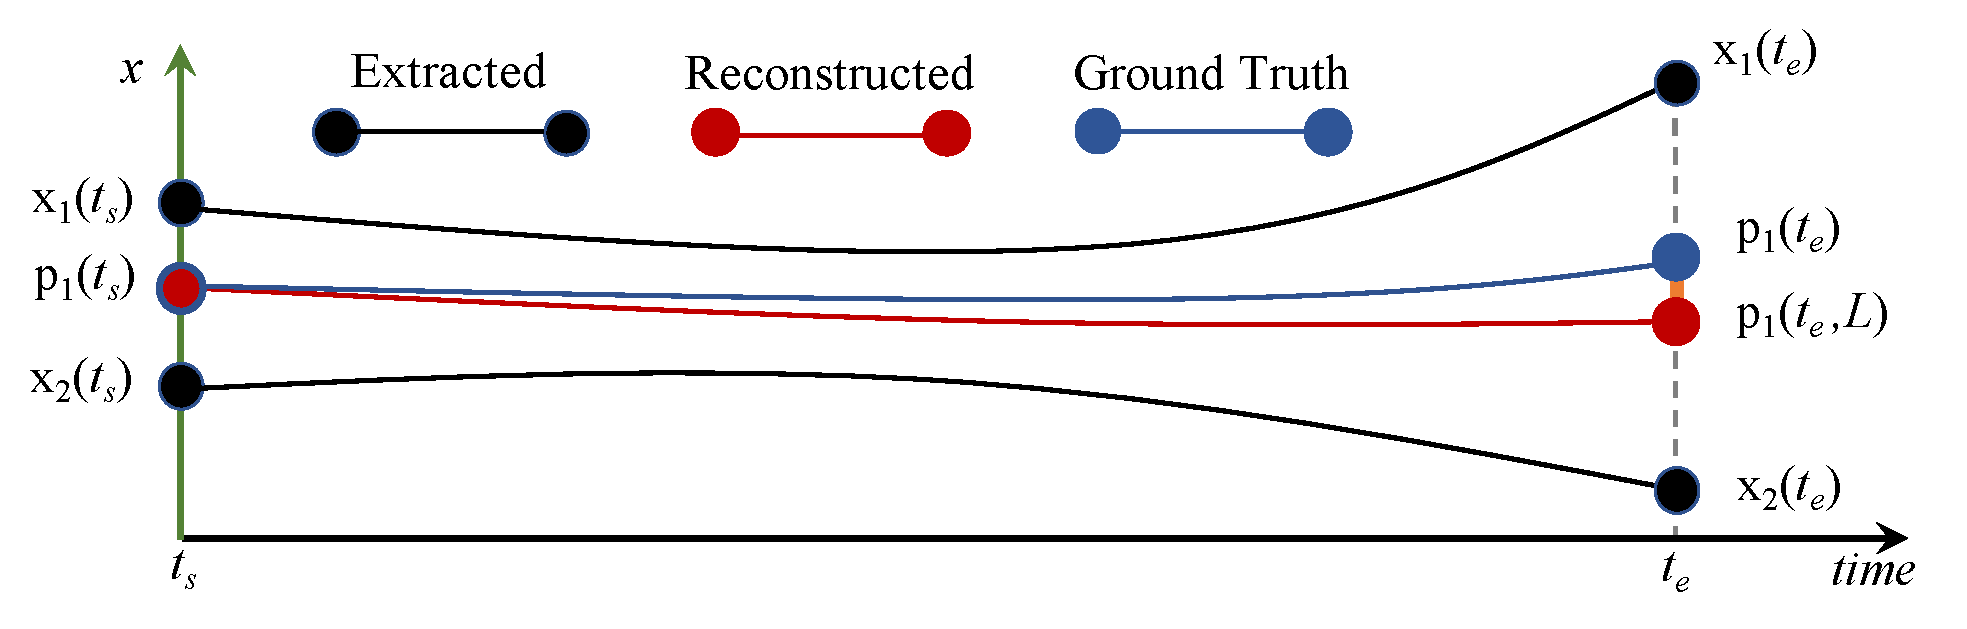
\includegraphics[width=0.9\linewidth]{Images/sample.pdf}
\vspace{-5mm}
\caption{Notional space-time visualization of Lagrangian representations for a time-varying 1D flow. The black trajectories are computed in situ and encode the behavior of the vector field between start time \textit{t$_{s}$} and end time \textit{t$_{e}$}. In a post hoc setting, a Lagrangian-based advection scheme \textit{L} is used to interpolate the extracted data and calculate the trajectory of a new particle p$_{1}$ . The red trajectory is the reconstructed trajectory and the blue trajectory is the ground truth.}
\vspace{-5mm}
\label{fig:sample}
\end{figure}

%First, we explore the use of Lagrangian representations to encode particle transport behavior of baryonic matter evolving under self-gravitating gas dynamics in the Nyx cosmology simulation~\cite{almgren2013nyx}.
%
%Next, we evaluate the potential of Lagrangian representations to encode the behavior of a fourth-order seismic wave propagation simulation SW4~\cite{petersson2015wave}. 
%
%In addition to investigating the use of Lagrangian representations for these vector fields, our study improves on prior efficacy and performance evaluations.
%
%We present the first statistical analysis of reconstruction accuracy for a range of spatiotemporal configurations as well as the first qualitative comparison to the traditional Eulerian approach. 
%
%Finally, we measure performance in a representative setting by considering integrated in situ infrastructure and execution using both GPUs and CPUs on a supercomputer.

%toring the time-varying vector field using a reduced Lagrangian representation is 
%
%In this paper, we focus on the axes of viability and efficacy. 
%
%Prior studies of reduced Lagrangian flow maps have shown improved accuracy-storage propositions compared to the traditional Eulerian paradigm under sparse temporal settings.
%
%However, only theoretical in situ settings, i.e., data sets are loaded from disk, on a single compute node or at small scale have been considered.
%
%With respect to type of time-varying vector field, either analytical data sets or data from climate and ocean modeling simulations has been considered.
%
%Further, for evaluation of reconstruction accuracy, comparisons to the Eulerian paradigm have been limited to quantitative analysis using a single average error.
%

%To determine viability, it is essential to evaluate the cost of in situ Lagrangian analysis in relation to the simulation execution time. 
%%
%In situ computation of a Lagrangian flow map, unlike the majority of in situ analysis tasks, requires computation and transfer of control between simulation and in situ analysis task every single cycle.
%%
%Our study integrates in situ infrastructure supporting Lagrangian analysis with simulation codes and evaluates execution on CPUs and GPUs on a modern supercomputer.
%%
%To contribute to research surrounding efficacy of the technique, we first consider three Exascale Computing Project simulation codes: a mini-application used for benchmarking, a wave propagation seismology simulation, and a Lyman-Alpha forest cosmology simulation, thus expanding our understanding across a variety of vector fields.
%%
%Next, we evaluate reconstruction accuracy by quantitatively measuring distribution of error across various configurations and present the first qualitative evaluation of the technique. 
%
%Overall, our study considers the current state-of-the-art of in situ Lagrangian analysis in representative high-performance computing settings, for two real-world simulation codes, with improved evaluations of viability and efficacy.
%%
%We believe this study is valuable to demonstrate the usage of the technique and serves to encourage adoption beyond theoretical research and climate and ocean modeling.


\section{Background and Related Work}
\label{sec:related}
\setlength{\belowdisplayskip}{3pt} \setlength{\belowdisplayshortskip}{3pt}
\setlength{\abovedisplayskip}{3pt} \setlength{\abovedisplayshortskip}{3pt}

\vspace{-1mm}
\subsection{Frames of Reference}
%
In fluid dynamics, there are two frames of reference to observe fluid motion: Eulerian and Lagrangian.
%
With the Eulerian frame of reference, the observer is in a fixed position.
%
With the Lagrangian frame of reference, the observer is attached to a fluid parcel and is moving through space and time.

%
Storage of a flow field in an Eulerian representation is typically done by means of its velocity field.
%
A velocity field $v$ is a time-dependent vector field that maps each point $x\in \mathbb R^d$ in space to the velocity of the flow field for a given time $t\in \mathbb R$
%
\begin{eqnarray}
{v} : \mathbb R^d \times \mathbb R \to \mathbb R^d,\; x,t \mapsto v(x,t)
\end{eqnarray}

%
In a practical setting, a flow field at a specific time/cycle is defined as vector data on a fixed, discrete mesh.
%
Time-varying flow is represented as a collection of such data over a variety times/cycles.


Storage of a flow field in a Lagrangian representation is done by means of its flow map $F_{t_0}^{t}$.
%
The flow map is comprised of the starting positions of massless particles $x_0$ at time $t_0$ and their respective trajectories that are interpolated using the time-dependent vector field.
%
Mathematically, a flow map is defined as the mapping
\begin{eqnarray}
F_{t_0}^{t}(x_0):\mathbb R \times \mathbb R \times \mathbb R^d \to \mathbb R^d,\; t \times t_0 \times x_0 \mapsto F_{t_0}^{t}(x_0) = x(t)
\end{eqnarray}
%
of initial values $x_0$ to the solutions of the ordinary differential equation
%
\begin{eqnarray}
\frac{d}{dt}x(t) = v(x(t),t)
\end{eqnarray}

In a practical setting, the flow map is represented as sets of particle trajectories calculated in the time interval $[t_0,t]\subset \mathbb R$.
%
The stored information, encoded in the form of known particle trajectories (i.e., a Lagrangian representation), encodes the behavior of the time-dependent vector field over an interval of time.
%

\vspace{-1mm}
\subsection{Lagrangian Analysis}
Within the vector field analysis and visualization community, Lagrangian methods have been increasingly researched in the past decade. 
%
In this paper, we focus on the use of Lagrangian methods to store time-varying vector fields in situ and enable subsequent post hoc analysis.
%The interest in Lagrangian representations is driven by their potential to offer reduced memory footprint and consequently enable post hoc analysis.
%
%fueled by temporal sparsity of data, i.e., simulations store data less frequently to avoid high storage costs.
%
In sparse temporal settings, Lagrangian representations are expected to perform better than their Eulerian counterparts, and the key intuition behind this is Lagrangian representations capture the behavior of the flow field over an interval of time, as opposed to the state at a single time slice.
%
However, in addition to the frequency of temporal sampling, the nature of the vector field and spatial sampling resolution impacts the quality of reconstruction.
%

Agranovsky et al.~\cite{agranovsky2014improved} conducted the seminal work to evaluate the efficacy of reduced Lagrangian representations.
%
To maintain domain coverage, the study proposed the use of uniform spatial sampling to extract sets of temporally non-overlapping basis trajectories.
%
Sane et al.~\cite{sane2018revisiting} studied performance across a range of spatiotemporal configurations when operating using a fixed storage budget.
%
%Pascal et al.~\cite{envirvis.20171099,siegfried2019tropical} used embedded routines to compute reduced Lagrangian data in order to explore coastal upwelling activity and visualized a derived scalar field representing trajectory density.
%However, a shortcoming of both studies is the measure of efficacy using a single quantitative average error for a limited set of applications.
%
The experiments in these works were conducted in a theoretical in situ setting, i.e., files were loaded from disk. %rather than integration with a simulation. 
%
%Such a theoretical set up fails to capture the cost of invoking in situ processing every cycle in a tightly-coupled system.
%
%
Most recently, Jakob et al.~\cite{Jakob20} train a DNN to upsample FTLE visualizations derived from reduced Lagrangian representations. 
%
To generate training data, they first compute Lagrangian representations of a 2D flow field using a tightly-coupled integration with an open source CFD solver on HPC resources and report in situ processing costs.
%
However, the grid size of $4\times4$ per rank used in the study is not representative of real-world applications.
%
Thus, current literature lacks in situ encumbrance measurements in representative settings.
%
%Our study explores this space by investigating the benefits and limitations of using reduced Lagrangian representations for previously unexplored time-varying vector fields.

%
%As such, prior works considering reduced Lagrangian representations have been restricted to analytical, ocean or climate data.
%

Lagrangian representations of a time-varying vector field can be extracted by adopting various strategies.
%
Sane et al.~\cite{sane2019interpolation} explored computing trajectories of variable duration and placement. 
%and consequently proposed a post hoc interpolation scheme to reduce reconstruction error by evaluating neighborhoods across interpolations.
%
Rapp et al.~\cite{rapp2019void} applied their void-and-cluster sampling technique to identify a representative set of scattered samples.
%
Although these strategies improved accuracy, they increased computation costs and are presently limited to single node settings.
%
To address scalability challenges of extracting a Lagrangian representation in distributed memory, Sane et al.~\cite{sane2020scalable} explored an accuracy-performance tradeoff and demonstrated the use of a communication-free model that stored only trajectories that remain within the rank domain during the interval of computation.
%

Prior works have presented research pertaining to post hoc reconstruction using Lagrangian-based interpolation schemes.
%
Hlawatsch et al.~\cite{hlawatsch2011hierarchical} proposed a hierarchical reconstruction scheme that can improve accuracy, but relies on access to data across multiple time intervals.
%
Chandler et al.~\cite{chandler2015interpolation} proposed a modified k-d tree as a search structure for Lagrangian data extracted from an SPH simulation.
%
Further, Chandler et al.~\cite{chandler2016analysis} identified correlations between Lagrangian-based interpolation error and divergence in the flow field.
%
Bujack et al.~\cite{bujack2015lagrangian} evaluated the use of parameter curves to fit interpolated pathline points to improve the aesthetic of trajectories calculated using Lagrangian data.
%
Lastly, Hummel et al.~\cite{hummel2016error} provided theoretical error bounds for error propagation that can occur when calculating trajectories using Lagrangian representations. 
%
%Finally, Jakob et al.~\cite{Jakob20} used DNNs to up-sample FTLE visualizations computed using reduced Lagrangian representations of 2D flow fields. 


\vspace{-1mm}
\subsection{Time-Varying Vector Field Reduction}
%Within the vector field analysis and visualization community, Lagrangian methods have been increasingly used in the past decade.
%
%Lagrangian coherent structures (LCS) are a popular technique to visualize attracting and repelling surfaces and were introduced by Haller et al~\cite{haller2001distinguished, haller2000lagrangian, haller2000finding}.
%
%The interest in the technique led to multiple efforts that were aimed at accelerating the computation and visualization of LCS~\cite{garth2007efficient,garth2009visualization,sadlo2007efficient,sadlo2011time}.
%
%LCS have also been used for uncertain transient vector field visualization by Guo et al.~\cite{guo2016finite}.
%
Although Eulerian representations have been shown to be susceptible to temporal sparsity~\cite{costa2004lagrangian}\cite{Qin2014}\cite{agranovsky2014improved}\cite{sane2018revisiting}, temporal subsampling remains the widely used solution to limit data storage.
%
Our study adds to this body of work by using temporal subsampling for comparison.
%
Multiple works have proposed single time step vector field reduction strategies while maintaining an Eulerian representation~\cite{lodha2000topology}\cite{lodha2003topology}\cite{theisel2003combining}\cite{tong2012salient}.
%
%Lodha et al.~\cite{lodha2000topology} controlled the compression of similar vectors into single vectors representing larger area.
%
%Further, Lodha et al.~\cite{lodha2003topology} proposed a top-down topology preserving compression technique.
%
%Theisel et al.~\cite{theisel2003combining} computed critical points and viewed the task as a mesh reduction, and later provided a threshold to filter important features~\cite{theisel2003compression}.
%
%With the objective of highlighting temporal features of the vector field, Tong et al.~\cite{tong2012salient} compressed the total amount of data steps stored by identifying key time steps.
%
Although these techniques could be used to reduce and store data more frequently, they do not inherently address the challenge of increasing temporal sparsity.
%

In a recent large-scale tornadic supercell thunderstorm study~\cite{atmos10100578}, Leigh Orf modified the I/O code to use a hierarchical data format and lossy floating-point compression via ZFP~\cite{lindstrom2006fast}.
%
ZFP provides dynamic accuracy control by allowing the user to specify a maximum amount of deviation.
%
Orf stated that although ZFP is effective for scalar fields that do not require differentiation during post hoc analysis, to maintain accurate vector field reconstruction, only a very small value of deviation can be chosen for each component of velocity.
%
Thus, ZFP allowed a limited amount of compression to time-varying vector field data without introducing significant uncertainty to post hoc analysis. 
%
The technique provided an average reduction of 30\% of total uncompressed vector field data, with regions of high gradient resulting in less compression. 
%
Overall, Orf referred to the use of lossy compression as unfortunate but necessary.

%In this paper, using the same temporal sampling frequency as the Lagrangian representations, we measure the reconstruction accuracy achieved by temporal subsampling for reference.
%Although these techniques are valuable, they do not sufficiently address the challenge of increasing temporal sparsity.
%
%\fix{I think we need a better statement here --- could reduce to get higher temporal sparsity.  And yet don't want to compare with that.}
%For a baseline comparison in our empirical study, we store data in an Eulerian representation at full resolution and use temporal subsampling.
%
%This paper presents an empirical study of the in situ encumbrance and performance tradeoffs when executing \textit{in situ Lagrangian analysis} in a practical setting, i.e., in situ on a supercomputer.


\section{In Situ Reduction via Lagrangian Representations}
\label{sec:method}
\begin{figure}[!t]
\centering
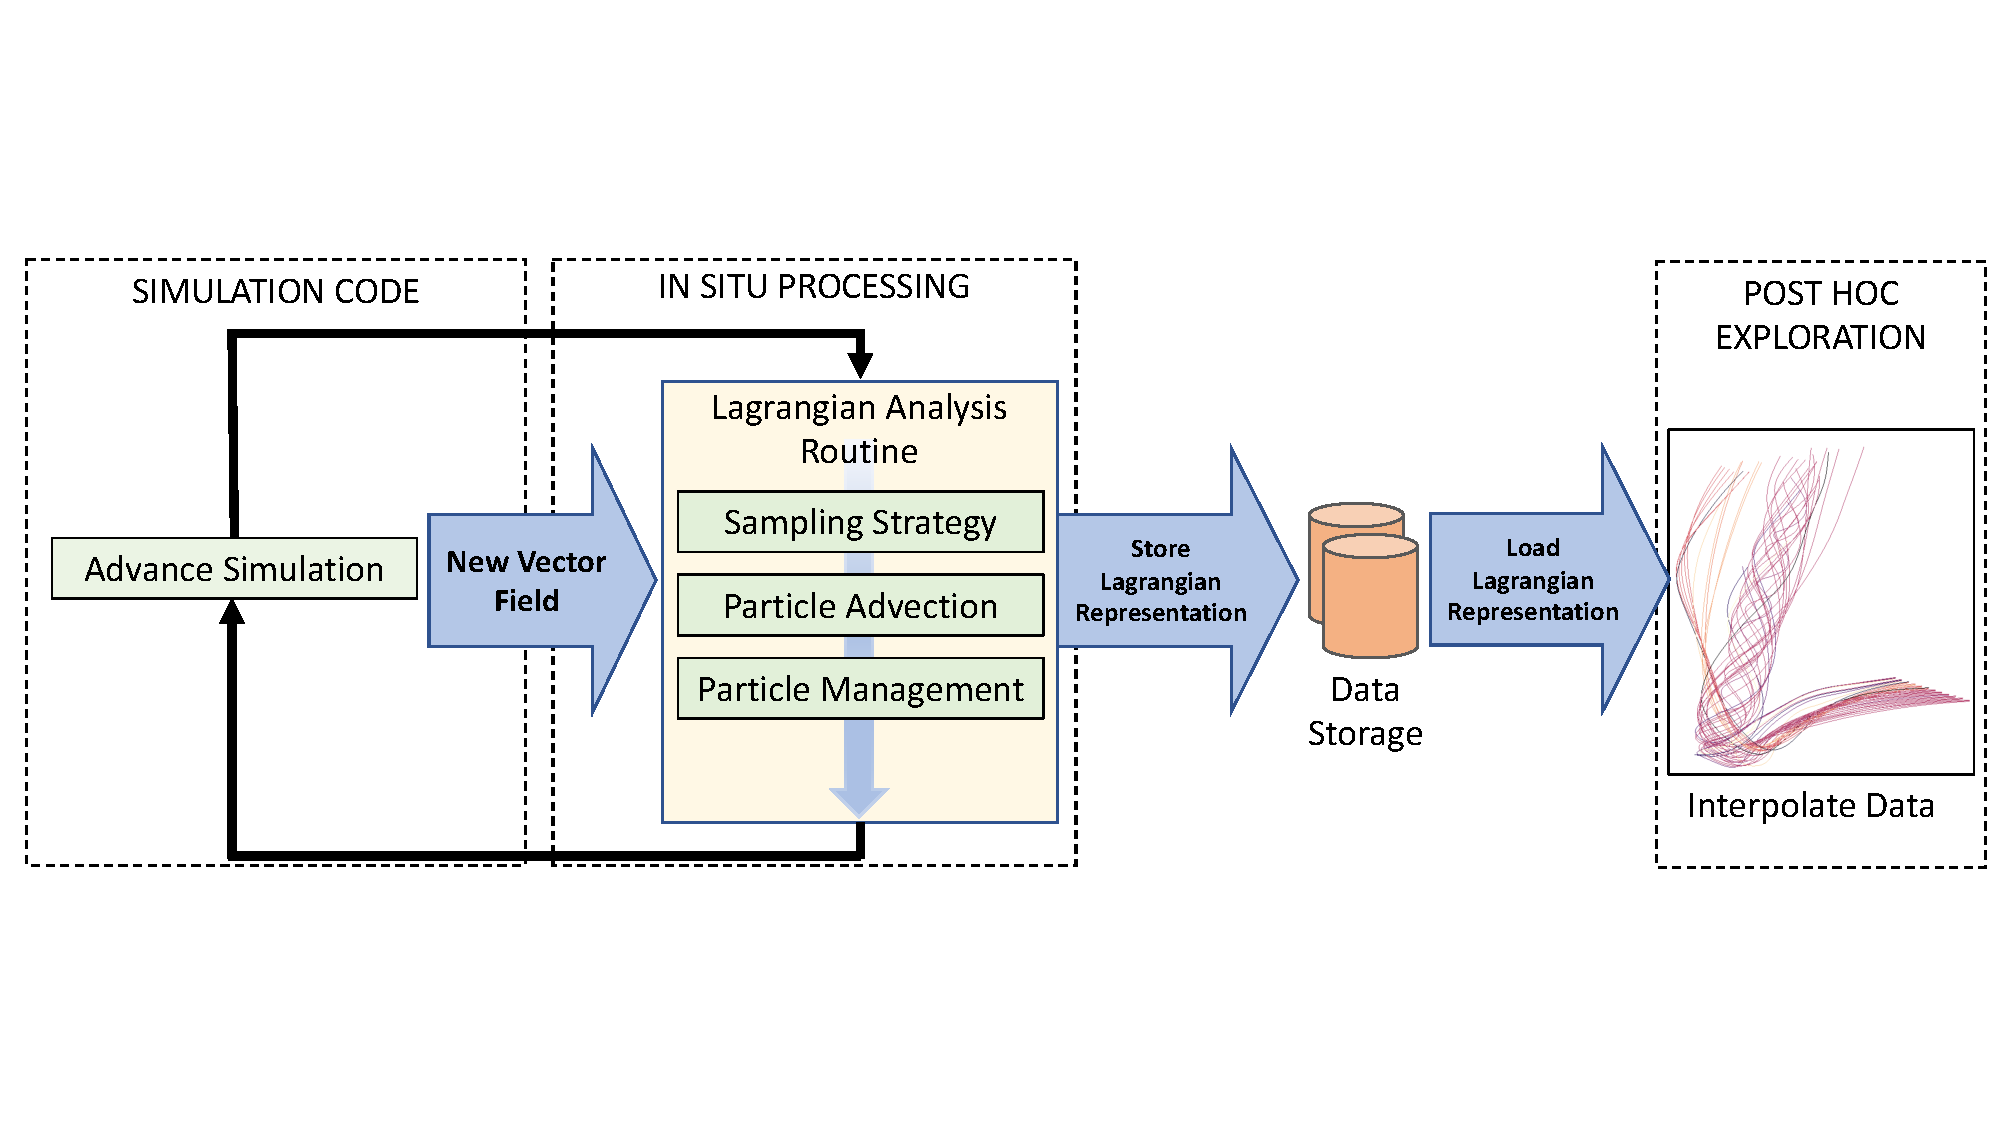
\includegraphics[width=0.9\linewidth,trim={0cm 4.3cm 0cm 4.3cm}, clip ]{Images/Schematic.pdf}
%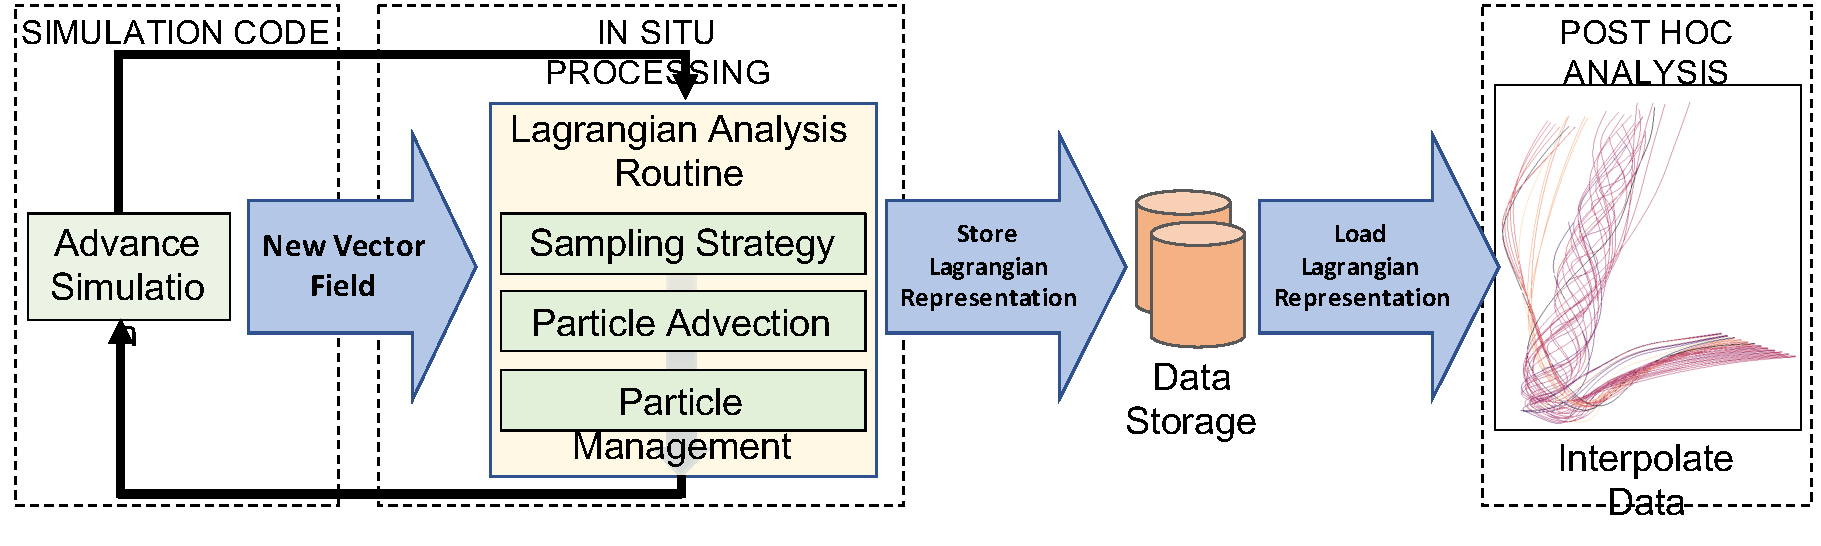
\includegraphics[width=0.9\linewidth]{Images/Schematic_Short.pdf}
\vspace{-2mm}
\caption{Schematic of the Lagrangian in situ reduction and post hoc exploration workflow.} %the simulation code with in situ processing integrated, data storage, and post hoc analysis.}
\vspace{-5mm}
\label{fig:schematic}
\end{figure}

%This section describes considerations for using and evaluating Lagrangian in situ reduction (L-ISR) for cosmology and seisomology time-varying vector fields. Specifically:
%\begin{tightItemize}
%\item Subsection~\ref{sec:instantiation} describes the instantiation we consider.
%\item Subsection~\ref{sec:evaluation} describes important evaluation criteria.
%\item Subsection~\ref{sec:workloads} describes important factors in defining workloads.
%\end{tightItemize}
%
%\subsection{Instantiation}
%\label{sec:instantiation}

This section describes the instantiation we consider for our study.
%
Figure~\ref{fig:schematic} shows a high-level description of the Lagrangian in situ reduction post hoc exploration (L-ISR-PHE) workflow. 
%
%There are many possible strategies for accomplishing the components within this workflow.
%
For our study, we focused on the current best practices in this space.
%
To describe our instantiation, the remainder of this section is divided based on the two phases: in situ reduction and post hoc exploration. 
%

\noindent\textbf{In Situ Reduction}
%In the in situ phase, for a data reduction operator without any a priori knowledge, a good strategy is to place samples such that domain coverage is maintained.
%
\fix{I love that you included this, but I think it is a distraction to
the reader.  Sadly, I propose you omit it.
}
Based on the in situ system classification in~\cite{childs2020terminology}, our L-ISR system classifies as one with a dedicated API integration, on node proximity, direct access, a time division of execution, automatic operation, and a derived output type.
%
\fix{Here is a possible replacement:
Both simulations we considered partitioned space amongst compute nodes,
with each compute node owning one portion of the vector field.
Our in situ routines followed this pattern, with an
instance of our Lagrangian analysis
routine running on each compute node, accessing its portion
of the vector field.
}
For our in situ data reduction strategy, we prioritized domain coverage.
\fix{I think the preceding sentence is a bit confusing.}
%
Similar to Agranovsky et al.~\cite{agranovsky2014improved}, we used uniform spatial sampling and a predetermined interval to store/reset particles.
%
Thus, we computed sets of temporally non-overlapping basis trajectories over the duration of the simulation.
%
%We refer to these trajectories as \textit{basis} trajectories.
%
Each set of basis trajectories encodes the behavior of the time-varying vector field over a specific interval of time.
%
%To introduce particles at the start of an interval, we use the uniform placement scheme by Agranovsky et al.~\cite{agranovsky2014improved}. 
%
%Using a uniform placement and resetting the particle trajectories after an interval helps maintain domain coverage and is simple to implement.
%
Our particle termination followed the local Lagrangian flow map model from Sane et al.~\cite{sane2020scalable}, where particles are terminated once they reach the end of the interval or exit the block.
%
Our implementation had two main knobs that control the total data storage and quality of reconstruction: number of basis trajectories, i.e., spatial sampling resolution, and frequency of storing information to disk, i.e., storage interval.
%
The effect of these settings varies depending on the underlying vector field. 
%
%We discuss these in~\ref{sec:workloads}.

We used the Ascent~\cite{Larsen2017Alpine} in situ infrastructure and VTK-m~\cite{moreland2016vtk} library to implement L-ISR. 
%
The Ascent API can be used to perform tightly-coupled integration with an application code and access various in situ analytics capabilities.
%%
The VTK-m Lagrangian filter on each rank operated independently and maintained its own list of particles.
%
We used the existing particle advection infrastructure available in VTK-m~\cite{pugmire2018performance}.
%
RK4 particle advection is implemented using VTK-m worklets (kernels) that offer performance portability by utilizing the underlying hardware accelerators.
%
In our implementation, each Lagrangian filter stored the displacement of each particle (three double), as well as its validity (one Boolean), i.e., whether the particle remained within the domain during the interval of calculation.
%
Overall, computing a Lagrangian representation increased the runtime memory cost on the simulation by approximately by four one-dimensional simulation ``fields''.
%
Simulations often have tens to hundreds of fields defined on the simulation grid, and thus, this cost would likely be acceptable for most simulations.
%
%In more complicated frameworks, it is possible to associate additional information (for example, ID, age, start location, previous locations, etc.) with each particle at the cost of higher runtime memory usage and data storage.
%

To compute a Lagrangian representation, the simulation invoked Ascent after every cycle it advanced.
%
Ascent accessed the simulation vector field data and consequently invoked the Lagrangian filter. 
%
The Lagrangian filter used the vector field to advance particles, and triggered the storage of trajectories at the end of an interval.
%
%In our implementation, following previous work~\cite{agranovsky2014improved}\cite{sane2018revisiting}\cite{sane2020scalable}, a trajectory in the Lagrangian representation is stored using a start and end location.
%
For integration, all the steps involved --- creating an instance of Ascent, specifying parameters, and invoking the VTK-m Lagrangian filter --- required only 23 lines of code (C++). % and less is a JSON input file was used.
%
%The code sample in Listing~\ref{lst:code} shows these steps. 
%

\noindent\textbf{Post Hoc Exploration}
For post hoc analysis, new particle trajectories are computed to explore the time-varying vector field. %by interpolating basis trajectories that were extracted in situ.
%
To construct new particle trajectories, we first identified which basis trajectories to follow and then performed interpolation.
%
Based on the study of accuracy of various Lagrangian-based advection schemes in~\cite{agranovsky2015subsampling}, our study employed a Delaunay triangulation to identify the neighborhood of valid basis trajectories and second-order barycentric coordinates for interpolation.
%
We used the CGAL~\cite{fabri2011cgal} library to construct and search the Delaunay triangulation.
%
After constructing new pathlines or deriving new scalar fields from the basis trajectories, we used VisIt~\cite{childs2012visit} to generate visualizations.

%\begin{lstlisting}[basicstyle=\footnotesize, label={lst:code}, caption=Ascent example., language=C++] 
%Ascent ascent;
%Node ascent_opts;
%ascent_opts[``runtime/type''] = ``ascent'';
%ascent.open(ascent_opts);
%conduit::Node mesh_data;
%conduit::Node pipelines;
%pipelines[``pl1/f1/type''] = ``lagrangian'';
%// filter knobs
%conduit::Node &lagrangian_params = pipelines[``pl1/f1/params''];
%lagrangian_params[``field''] = ``velocity'';
%lagrangian_params[``step_size''] = 0.02; 
%lagrangian_params[``storage_interval''] = 25; 
%lagrangian_params[``seed_resolution''] = 8; 
%conduit::Node actions;
%conduit::Node &add_pipelines = actions.append();
%add_pipelines[``action''] = ``add_pipelines'';
%add_pipelines[``pipelines''] = pipelines;
%conduit::Node &execute  = actions.append();
%execute[``action''] = ``execute'';
%conduit::Node &reset  = actions.append();
%reset[``action''] = ``reset'';
%ascent.publish(mesh_data);
%ascent.execute(actions);
%ascent.close();
%\end{lstlisting}
%
%
%We use Ascent to store the complete velocity field at a specified frequency in order to evaluate the traditional Eulerian paradigm.
%
%For every Eulerian configuration, we store the full spatial resolution of the simulation domain under consideration.
%

%\subsection{Evaluation Criteria}
%\label{sec:evaluation}
%In this study, we consider the following four evaluation criteria (EC) across the workflow:
%%
%\begin{tightEnumerate}
%\item\textbf{(EC1) In situ reduction time:} the execution time spent by the simulation on data analysis and visualization.
%\item\textbf{(EC2) In situ reduction memory:} the runtime memory used by in situ processing.
%\item\textbf{(EC3) Data storage size:} the file storage costs (i.e., bytes).
%\item\textbf{(EC4) Post hoc exploration accuracy:} the quantitative and qualitative accuracy of new interpolated trajectories or derived fields.
%\end{tightEnumerate}
%%
%
%\subsection{Workload Factors}
%\label{sec:workloads}
%To understand the performance characteristics of L-ISR, we identified four parameters that when varied produce the workloads we want to evaluate for our study:
%\begin{tightEnumerate}
%\item\textbf{(WF1) Number of basis particles:} 
%%We vary the number of basis particles initialized per rank. The number of basis trajectories impacts the cost of particle advection every cycle of the simulation, the size of the data stored to disk and the accuracy of the reconstruction. 
%%
%We specify the number of particles initialized using the notation $\textbf{1:X}$, where X is the reduction factor. For example, a 1:8 configuration states that one particle is used for every 8 grid points (12.5\% of the original data size). WF1 impacts every EC.
%\item\textbf{(WF2) Storage interval:} 
%%We consider the frequency at which files are stored to disk. Additionally, for the Lagrangian representation, the interval is equal to the integration length of each particle, and can thus, be consequential to the accuracy of reconstruction. 
%%
%We use $\textbf{I}$ to denote storage interval. WF2 impacts EC3 and EC4. 
%\item\textbf{(WF3) Grid size:} 
%%We consider different grid sizes to measure the in situ encumbrance of varying workloads. In particular, we are interested in the in situ encumbrance when a single compute node is operating on a large number of grid points. An additional benefit of varying the grid size is insight into the variation in simulation cycle time and consequently the percentage of time spent on in situ processing. 
%WC3 impacts EC1, EC2, and EC3. 
%\item\textbf{(WF4) Concurrency:} We consider the costs at multiple scales (i.e., number of compute nodes, MPI ranks). Further, the simulation codes described in \ref{sec:simulations} required different parallelization hardware, and thus, between simulation codes we measure the costs of Lagrangian representation extraction using, both, GPUs and CPUs for particle advection. WF4 impacts EC1 and EC2.
%\end{tightEnumerate}


\section{Study Overview}
\label{sec:study}
This section provides an overview of our study. It is organized as follows: runtime environment~(\ref{sec:runtime}), simulation codes~(\ref{sec:simulations}), experiments~(\ref{sec:experiments}), and evaluation metrics~(\ref{sec:metrics}). %, and runtime environment~(\ref{sec:runtime}).

\subsection{Runtime Environment}
\label{sec:runtime}
Our study used the Summit supercomputer at ORNL.
%
A Summit compute node has two IBM Power9 CPUs, each with 21 cores running at 3.8 GHz and 512 GBytes of DDR4 memory.
%
Nodes on Summit also have enhanced on-chip acceleration with each CPU connected via NVLink to 3 GPUs, for a total of 6 GPUs per node.
%
Each GPU is an NVIDIA Tesla V100 with 5120 CUDA cores, 6.1 TeraFLOPS of double precision performance, and 16 GBytes of HBM2 memory.
%
Lastly, it has a Mellanox EDR 100G InfiniBand, Non-blocking Fat Tree as its interconnect topology.

\subsection{Simulation Codes}
\label{sec:simulations}
We focused our study on 
%two 
computational science applications being developed as part of the US Department of Energy Office of Science Exascale Computing Project (ECP).
%
%See additional material for benchmarking on a third application: the Cloverleaf3D ECP proxy simulation code~\cite{mallinson2013cloverleaf}.
%that solves compressible Euler equations in a hydrodynamics setting on a Cartesian grid using an explicit second-order method. 
%
%Cloverleaf3D has been developed and used by several studies to evaluate emerging architectures and various techniques targeting Exascale applications.

\textbf{Nyx:} In this cosmological simulation~\cite{almgren2013nyx}, baryonic matter is evolved by solving the equations of self-gravitating gas dynamics.
%
The simulation involves particles gravitating toward high-density regions to form multiple clusters across the domain. 
%
%For this simulation, we derived the velocity field using the fields of momentum and density of the gas.
%
One of the features of interest is the distribution of high densities clusters.
%
To study the distribution, scientists currently perform statistical analysis of gas particle density at a single time slice.
%
We investigated the potential of reduced Lagrangian representation to accurately visualize the particle evolution and the distribution of high-density clusters using pathlines.
%
At the time of this study, the Nyx simulation executes using the CPU on a single Summit compute node.
%
For this simulation, we performed L-ISR using the CPU.

\textbf{SW4:} In this seismology simulation~\cite{petersson2015wave}, seismic wave propagation is studied using a fourth-order method.
%
The application simulates waves radiating from the epicenter through viscoelastic media. 
%
The simulation produced multiple distinct spatial domains with a time-varying 3D displacement field.
%
We operated on a single domain and used the displacement vector as input.
%
We investigated how accurately we can derive and visualize the field encoding displacement over time in two regions: at the epicenter and away from the epicenter.
%
At the time of this study, the SW4 simulation scales to a large number of ranks across several compute nodes and uses GPUs for execution on Summit.
%
For this simulation, we performed L-ISR using GPUs.
%

\textbf{Cloverleaf3D:} We include a third mini-application for a benchmarking study. The Cloverleaf3D ECP proxy simulation code~\cite{mallinson2013cloverleaf} solves compressible Euler equations in a hydrodynamics setting on a Cartesian grid using explicit second-order method.
%
Cloverleaf3D has been developed and used by several studies to evaluate emerging architectures and various techniques targeting Exascale applications.

%
\subsection{Experiments}
\label{sec:experiments}

For each application in this study, we organize our experiments to inform in situ encumbrance and post hoc efficacy. 
%
We consider four evaluation criteria (EC).
%
To inform in situ encumbrance,  we measure the execution time (EC1) and runtime memory (EC2) requirements of in situ processing.
%
To inform post hoc efficacy, we measure the size of data artifacts (EC3) and the accuracy of post hoc analysis (EC4).
%\begin{tightEnumerate}
%\item\textbf{(EC1) In situ reduction time:} the execution time spent by the simulation on data analysis and visualization.
%\item\textbf{(EC2) In situ reduction memory:} the runtime memory used by in situ processing.
%\item\textbf{(EC3) Data storage size:} the file storage costs (i.e., bytes).
%\item\textbf{(EC4) Post hoc exploration accuracy:} the quantitative and qualitative accuracy of new interpolated trajectories or derived fields.
%\end{tightEnumerate}

Next, we identify four factors that when varied produce the workloads we want to evaluate for our study:
\begin{tightItemize}
\item\textbf{Number of particles:} the spatial sampling resolution denoted using \textbf{1:X}, where X is the reduction factor. For example, a 1:8 configuration states that one basis particle is used for every 8 grid points ($\approx$12.5\% of the original data size).  
\item\textbf{Storage interval:} the number of cycles between saves and denoted by \textbf{I}.
\item\textbf{Grid size:} the resolution of the mesh. 
\item\textbf{Concurrency:} the scale of execution and parallelization hardware.
\end{tightItemize}
%
%For each application, in response to our evaluation criteria, we organize our experiments to inform in situ encumbrance (EC1, EC2) and post hoc efficacy (EC3, EC4). 
%
Rather than consider a complete cross-product of options for every workload factor, we sample the space of possible options.
%
Our goal was to simultaneously provide coverage and yet allow us to see the impact of certain workload factors, all while staying within our compute budget.
%
For Nyx, we ran a total of 18 experiments, with 6 informing in situ encumbrance (varying \textbf{1:X}, grid size) and 12 informing post hoc efficacy (varying \textbf{1:X}, \textbf{I}).
%
For SW4, we ran a total of 11 experiments, with 7 informing in situ encumbrance (varying \textbf{1:X}, grid size, concurrency) and 4 informing post hoc efficacy (varying \textbf{1:X}).
%
The specific options selected are presented along with the results in Section~\ref{sec:results}. 
%details of 
%\begin{table}
%\parbox{.495\linewidth}{
%\centering
%\scalebox{0.9}{
%\begin{tabular}{|r||c|c|c|c|c|}
%\hline
%Simulation Code & SW4 & Nyx \\ \hline
%\# of Particles  & 3 & 3 \\
%Interval & 1 & 1 \\
%Grid Size & 3,2 & 2 \\
%Concurrency & 2 & 1 \\  \hline
%Total Experiments & 7 & 6 \\ \hline
%\end{tabular}
%}
%%\caption{}
%%\caption{\label{tab:campaign1}Experimental overview to inform the \textit{in situ} encumbrance.  *For SW4, we were able to run a very fine grid size at low concurrency, but not the entire cross product of options due to limitations in compute time.  Overall, we considered 13 experiments.}
%}
%\hfill
%\parbox{.495\linewidth}{
%\scalebox{0.9}{
%\begin{tabular}{|r||c|c|c|c|c|}
%\hline
%Simulation Code & SW4 & Nyx \\ \hline
%\# of Particles  & 4 & 3 \\
%Interval & 1 & 4 \\
%Grid Size & 1 & 1 \\
%Concurrency & 1 & 1 \\  \hline
%Total Experiments & 4 & 12 \\ \hline
%\end{tabular}
%}
%%\caption{}
%%\caption{\label{tab:campaign2}Experimental overview to inform the post hoc efficacy.
%%
%%Overall, we considered 16 experiments.}
%}
%\caption{}
%\end{table}
%
%\begin{table}[h]
%\centering
%\scalebox{0.9}{
%\begin{tabular}{|r||c|c|c|c|c|}
%\hline
%Simulation Code & SW4 & Nyx \\ \hline
%\# of Particles  & 3 & 3 \\
%Interval & 1 & 1 \\
%Grid Size & 3,2 & 2 \\
%Concurrency & 2 & 1 \\  \hline
%Total Experiments & 7 & 6 \\ \hline
%\end{tabular}
%}
%\caption{\label{tab:campaign1}Experimental overview to inform the \textit{in situ} encumbrance.  *For SW4, we were able to run a very fine grid size at low concurrency, but not the entire cross product of options due to limitations in compute time.  Overall, we considered 13 experiments.}
%\end{table}
%
%\begin{table}[h]
%\centering
%\scalebox{0.9}{
%\begin{tabular}{|r||c|c|c|c|c|}
%\hline
%Simulation Code & SW4 & Nyx \\ \hline
%\# of Particles  & 4 & 3 \\
%Interval & 1 & 4 \\
%Grid Size & 1 & 1 \\
%Concurrency & 1 & 1 \\  \hline
%Total Experiments & 4 & 12 \\ \hline
%\end{tabular}
%}
%\caption{\label{tab:campaign2}Experimental overview to inform the post hoc efficacy.
%%
%Overall, we considered 16 experiments.}
%\end{table}


\subsection{Evaluation Metrics}
\label{sec:metrics}
We select our evaluation metrics based on the evaluation criteria listed in Section~\ref{sec:experiments}.
%

For EC1, we measure \textbf{Step}, the average cost of invoking the Lagrangian VTK-m filter through Ascent every cycle in seconds. Additionally, we present the percentage of simulation time spent on data analysis and visualization, or \textbf{DAV\%}.
%
We use \textbf{Sim$_{cycle}$} to denote the average time required for a single simulation cycle in seconds.

For EC2, we measure \textbf{InSituMem}, the runtime memory cost incurred by every compute node to maintain the state (current position) of particles at runtime in Bytes.
%

For EC3, we limit our measurement and discussion of I/O to the total data storage~(or \textbf{DS}) required on the file system and report it in Bytes stored.
%
We do not report or factor the cost of I/O write times. 
%
Besides being an infrequently performed operation, we observed that for the scale of study we conducted that Summit provides very fast write times.
%
In comparison to performing in situ processing every cycle, we found the I/O write cost to be negligible at the scale we test.
%Given the range of files sizes stored to disk by a single MPI rank in our study is between 0.5MB to 115MB, we believe the I/O write cost is negligible at the scale we test.

For EC4, we consider both a statistical and qualitative analysis. 
%
We use the post hoc efficacy of various Eulerian configurations storing full-resolution meshes at varying storage intervals as a reference for comparison.
%
To measure the error of each reconstructed trajectory (Lagrangian and Eulerian), we calculate the average Euclidean distance of interpolated points from the ground truth~(precomputed using the complete simulation data).
%
We visualize distributions using violin plots with included boxplots to capture interquartile ranges.
%
Our qualitative comparisons for both applications involve visualizing reconstructed time-varying vector fields using pathlines or derived scalar fields and observing the preservation of features of interest.
%
%
%We then visualize the distribution of reconstruction error across particles using violin plots with included boxplots to capture interquartile ranges.
%
%Similarly, for SW4, we first derive a displacement magnitude field from reconstructed trajectories and then visualize the distribution of displacement in comparison to the ground truth.
%
%Our qualitative comparisons for both applications involve visualizing reconstructed time-varying vector fields using pathlines or derived scalar fields and observing the preservation of features of interest.



\section{Results}
\label{sec:results}
Our results are organized as follows.
%
Sections~\ref{sec:nyx} and\ref{sec:sw4} present findings from our study investigating reduced Lagrangian representations for cosmology and seismology applications, respectively.
%
%Section~\ref{sec:cloverleaf3d} contains results from our benchmarking study.
%
%We organize our results by discussing the use of Lagrangian representations for the cosmology and seismology () applications, and  .
%
Tables~\ref{table:nyx_encumbrance} and~\ref{table:sw4_encumbrance} provide information pertaining to in situ encumbrance experiments, such as concurrency information, spatial dimensions, Sim$_{cycle}$, number of particles, \textbf{InSituMem}, \textbf{Step}, and \textbf{DAV\%}, for each application. 
%
Figure~\ref{fig:insitucost} contains the execution time per cycle for all the in situ encumbrance experiments. %from both applications.  
%
\begin{figure}[!b]
\centering
\vspace{-4mm}
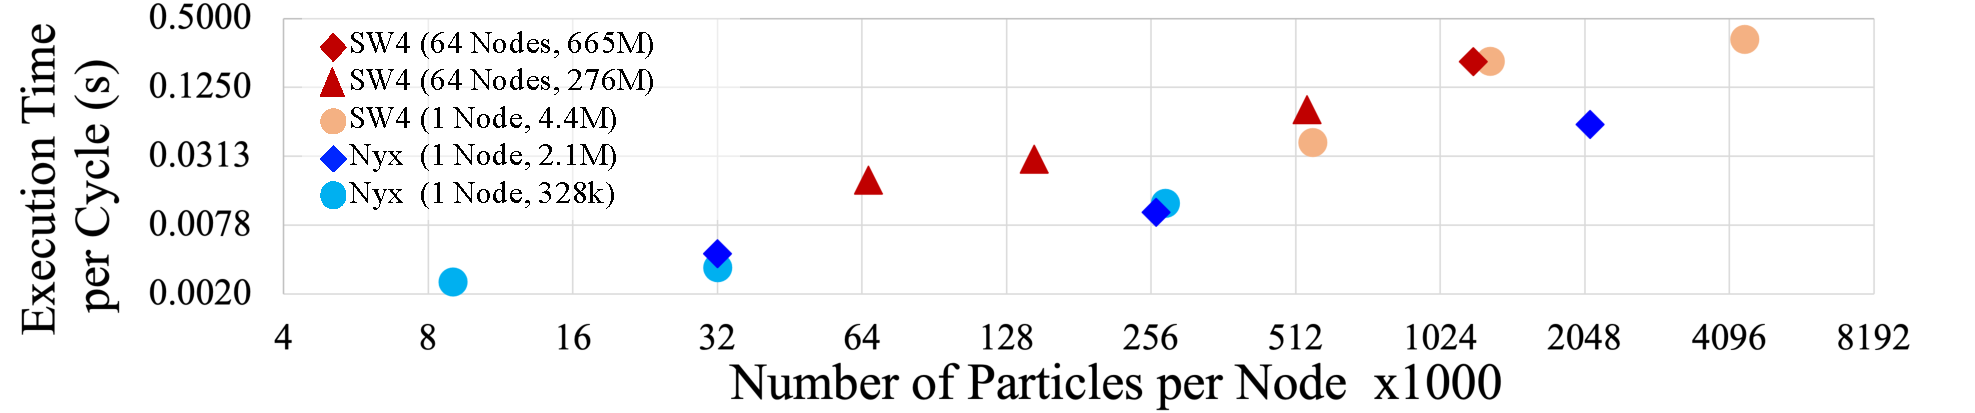
\includegraphics[width=\linewidth]{Images/InSituCost_Stretch2.pdf}
%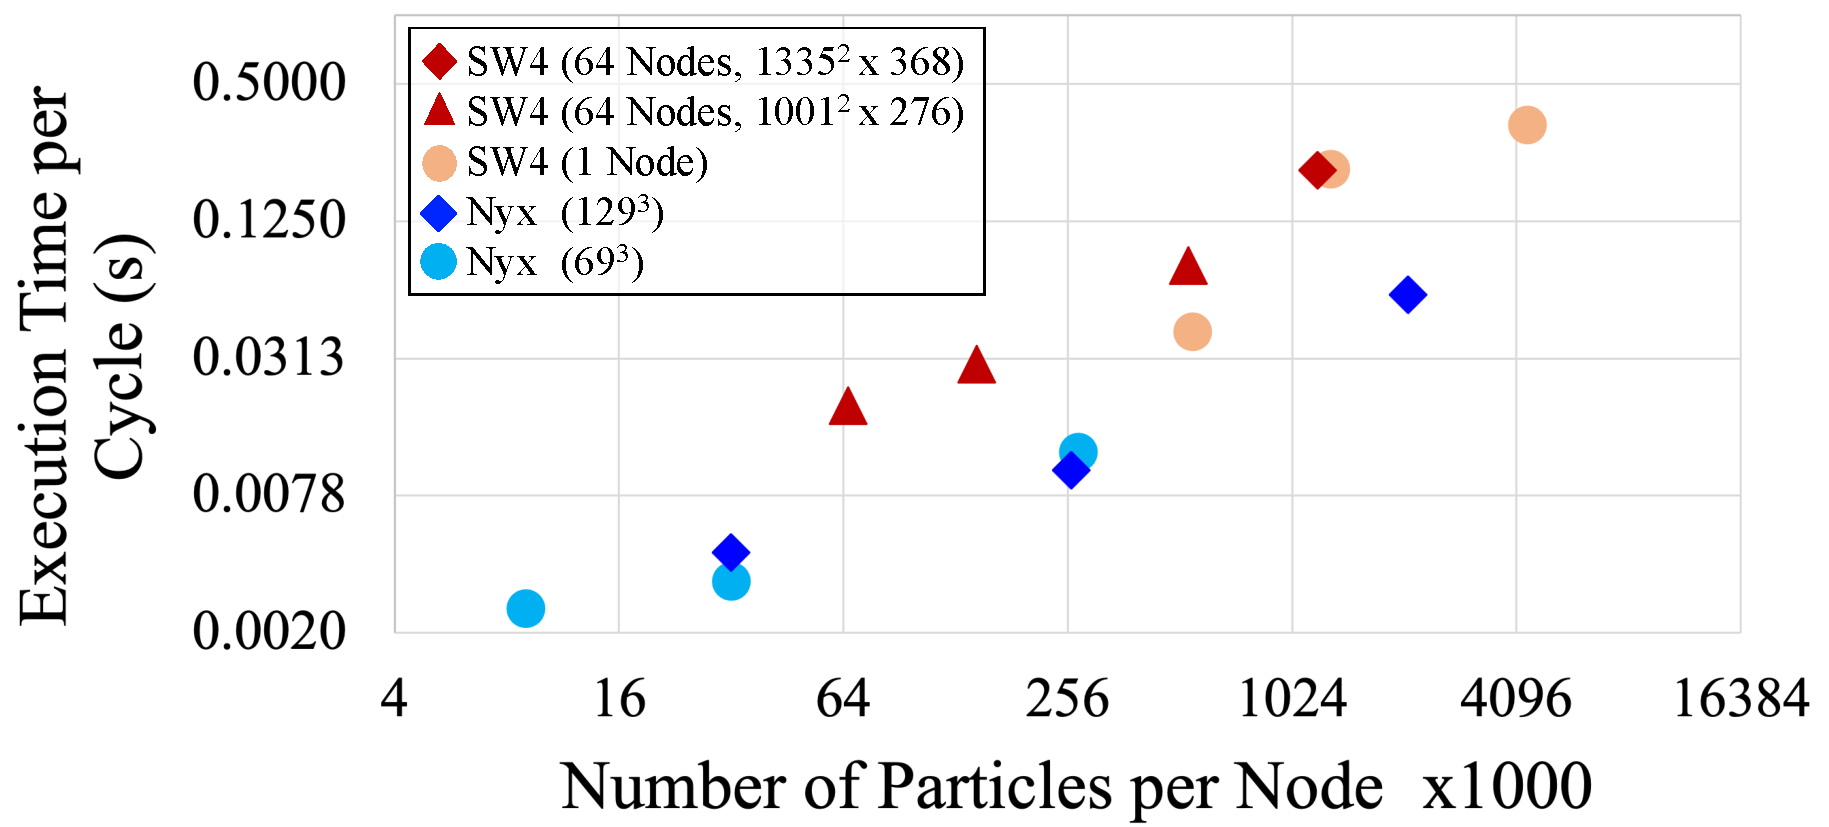
\includegraphics[width=0.7\linewidth]{Images/InSituCost.pdf}
\vspace{-5mm}
\caption{Lagrangian in situ reduction cost per cycle for all in situ encumbrance experiments. The SW4 simulation executes with six ranks (each allocated one GPU) sharing memory on every node. The Nyx simulation executes on a single rank using all the cores of two CPUs on a single node. The legend includes concurrency and number of simulation grid points in parenthesis and both axes use logarithmic scales.} 
\vspace{-5mm}
\label{fig:insitucost}
\end{figure}

%
Figures~\ref{fig:nyx_violinplot},~\ref{fig:nyx_figure},~\ref{fig:sw4_violinplot}, and ~\ref{fig:sw4_figure} show the results of our post hoc efficacy evaluation.
%
For each application, the figures are annotated with configuration specifics such as the \textbf{DS}, \textbf{1:X}, and \textbf{I}.
%
Further, Lagrangian and Eulerian tests are distinguished explicitely in the captions or are labeled L$T$ and E$T$, respectively, where $T$ is the test number.
%
%We refer to these tables and figures in the discussion that follows. 

\vspace{-1mm}
\subsection{Nyx Cosmology Simulation}
\label{sec:nyx}
\noindent\textbf{In Situ Encumbrance}
Using all the cores of two CPUs on a single compute node, we used OpenMP to parallelize the Nyx simulation and Lagrangian VTK-m filter.
%
We tested two options for grid size - $69^{3}$ and $129^{3}$ - on a single rank, and three particle advection workloads (1:1, 1:8, 1:27) each.
%
In a single compute node hour, the simulation performed approximately 300 and 38 cycles, when using $69^{3}$ and $129^{3}$ grid sizes, respectively.
%
%In a single compute node hour, the simulation performs approximately 300 cycles for the $69^{3}$ resolution and approximately 38 cycles for the $129^{3}$ resolution.
%
An 8X increase in grid size results in a proportional increase in Sim$_{cycle}$ but only a small increase in particle advection costs for the same number of particles.
%
We expect a single rank to operate on between $32^{3}$ to $256^{3}$ grid resolutions, and thus our workloads provide a representative estimate of \textbf{DAV\%}.
%
%For example, sampling a $256^{3}$ using a 1:8 reduction involves computing 2.1M basis trajectories. 

An encouraging finding is the low in situ encumbrance when performing L-ISR on the CPUs.
%
Depending on the setup of various simulations and the form of integration for in situ processing, future work can consider offloading L-ISR computation to CPUs.
%
Overall, considering the longer Sim$_{cycle}$ times for the Nyx simulation, and parallel compution coupled with low memory latency when using CPUs, the highest in situ encumbrance to extract a Lagrangian represenation was 0.1\% of the simulation time or under 0.06s to compute 2.1M basis trajectories per cycle.\\
\begingroup
\setlength{\tabcolsep}{-2pt}
%\renewcommand{\arraystretch}{1} % Default value: 1
\begin{table*}[!t]
%\centering
\begin{tabular}{|P{1.1cm}|P{1.1cm}|P{2.7cm}|P{1.3cm}|P{1.5cm}|P{1.9cm}|P{1.7cm}|P{1.7cm}|}
\hline
Nodes & Ranks & Dimensions & \textbf{Sim$_{cycle}$} & Particles & \textbf{InSituMem} & \textbf{Step} & \textbf{DAV\%} \\ 
% & Ranks & & & /Node & /Node (MB) & & \\ 
\hline
%\multicolumn{9}{l}{} & \\
%\multicolumn{9}{l}{\textbf{          Cloverleaf3D Proxy Hydrodynamics Application }} \\ %& \multirow{13}{*}{\includegraphics[width=0.93\linewidth]{images/GPU_Step.pdf}}\\
%\cline{1-9}
%\multirow{9}{*}{16} & \multirow{9}{*}{96} & \multirow{9}{*}{$586\times586\times586$} & 20 & 4.73 & \multirow{3}{*}{1.5M} & \multirow{3}{*}{40.2 } & 0.4475 & 9.408 \\
%\cline{4-4}
%& & & 40 & 4.08 & & & 0.3221 & 7.894 \\
%\cline{4-4}
%& & & 60 & 4.39 & & & 0.3838 & 8.742 \\
%\cline{4-6}%\cline{6-6}
%& & & 20 & 4.50 & \multirow{3}{*}{474k} & \multirow{3}{*}{12 } & 0.1882 & 4.182 \\
%\cline{4-4}
%& & & 40 & 4.14 & & & 0.1628 & 3.932 \\
%\cline{4-4}
%& & & 60 & 4.33 & & & 0.1498 & 3.459 \\
%\cline{4-6}%\cline{6-6}
%& & & 20 & 4.19 & \multirow{3}{*}{186k} & \multirow{3}{*}{4.2 } & 0.0925 & 2.207 \\
%\cline{4-4}
%& & & 40 & 4.11 & & & 0.1043 & 2.537 \\
%\cline{4-4}
%& & & 60 & 3.87 & & & 0.0830 & 2.144 \\
%\cline{1-9}
%%\multicolumn{9}{l}{} & \\
%\multicolumn{8}{l}{\textbf{          SW4 Seismic Modeling Simulation }}\\
%\cline{1-8}
%\multirow{3}{*}{1} & \multirow{3}{*}{6} & $251\times251\times70$ & 0.35s & 555k & 13.89MB & 0.0412s & 11.67\% \\
%%\cline{3-3}\cline{5-6}
%& & $335\times335\times93$  & 2.02s & 1.3M & 33.16MB & 0.2125s & 10.48\% \\
%%\cline{3-3}\cline{5-6}  
%& & $501\times501\times139$  & 7.58s & 4.4M & 111.13MB & 0.3309s & 4.365\% \\ %& \multirow{13}{*}{\includegraphics[width=0.93\linewidth]{images/CPU_Step.pdf}}\\
%\cline{1-3}%\cline{5-6}
%\multirow{4}{*}{64} & \multirow{4}{*}{384} & \multirow{3}{*}{$1001\times1001\times276$} & 1.6s & 66k & 1.6MB & 0.0194s & 1.201\% \\
%%\cline{6-6}
%& & & 1.5s & 146k & 3.6MB & 0.0295s & 1.944\% \\
%%\cline{6-6}
%& & & 1.3s & 540k & 13.5MB & 0.0798s & 6.175\% \\
%\cline{3-3}%\cline{5-6}
%& & $1335\times1335\times368$ & 2.9s & 1.2M & 31.9MB & 0.2095s & 7.074\% \\
%\cline{1-8}
%%\multicolumn{9}{l}{} \\
%\multicolumn{8}{l}{\textbf{          Nyx Cosmology Simulation }} \\
\cline{1-8}
\multirow{6}{*}{1} & \multirow{6}{*}{1} & \multirow{3}{*}{$65\times65\times65$} & \multirow{3}{*}{10.9s} & 9k & 0.2MB & 0.0025s & 0.023\% \\
%\cline{6-6}
& & & & 32k & 0.8MB & 0.0033s & 0.030\% \\
%\cline{6-6}
& & & & 274k & 6.8MB & 0.0122s & 0.0112\% \\
\cline{3-3}%\cline{5-6}
& & \multirow{3}{*}{$129\times129\times129$} & \multirow{3}{*}{88.3s} & 78k & 1.9MB & 0.0044s & 0.005\% \\
%\cline{6-6}
& & & & 262k & 6.5MB & 0.0101s & 0.011\% \\
%\cline{6-6}
& & & & 2.1M & 53.6MB & 0.0596s & 0.067\% \\
\hline
\end{tabular}
\caption{\textit{In situ} encumbrance evaluation and experiment configurations for the Nyx simulation executing on CPUs. The in situ cost of computing Lagrangian representations every cycle~(\textbf{Step}) remains low in comparison to the average simulation cycle time~(\textbf{Sim$_{cycle}$}) resulting in low \textbf{DAV\%}.}
\vspace{-5mm}
\label{table:nyx_encumbrance}
\end{table*}
\endgroup

\begin{figure}[!t]
\centering
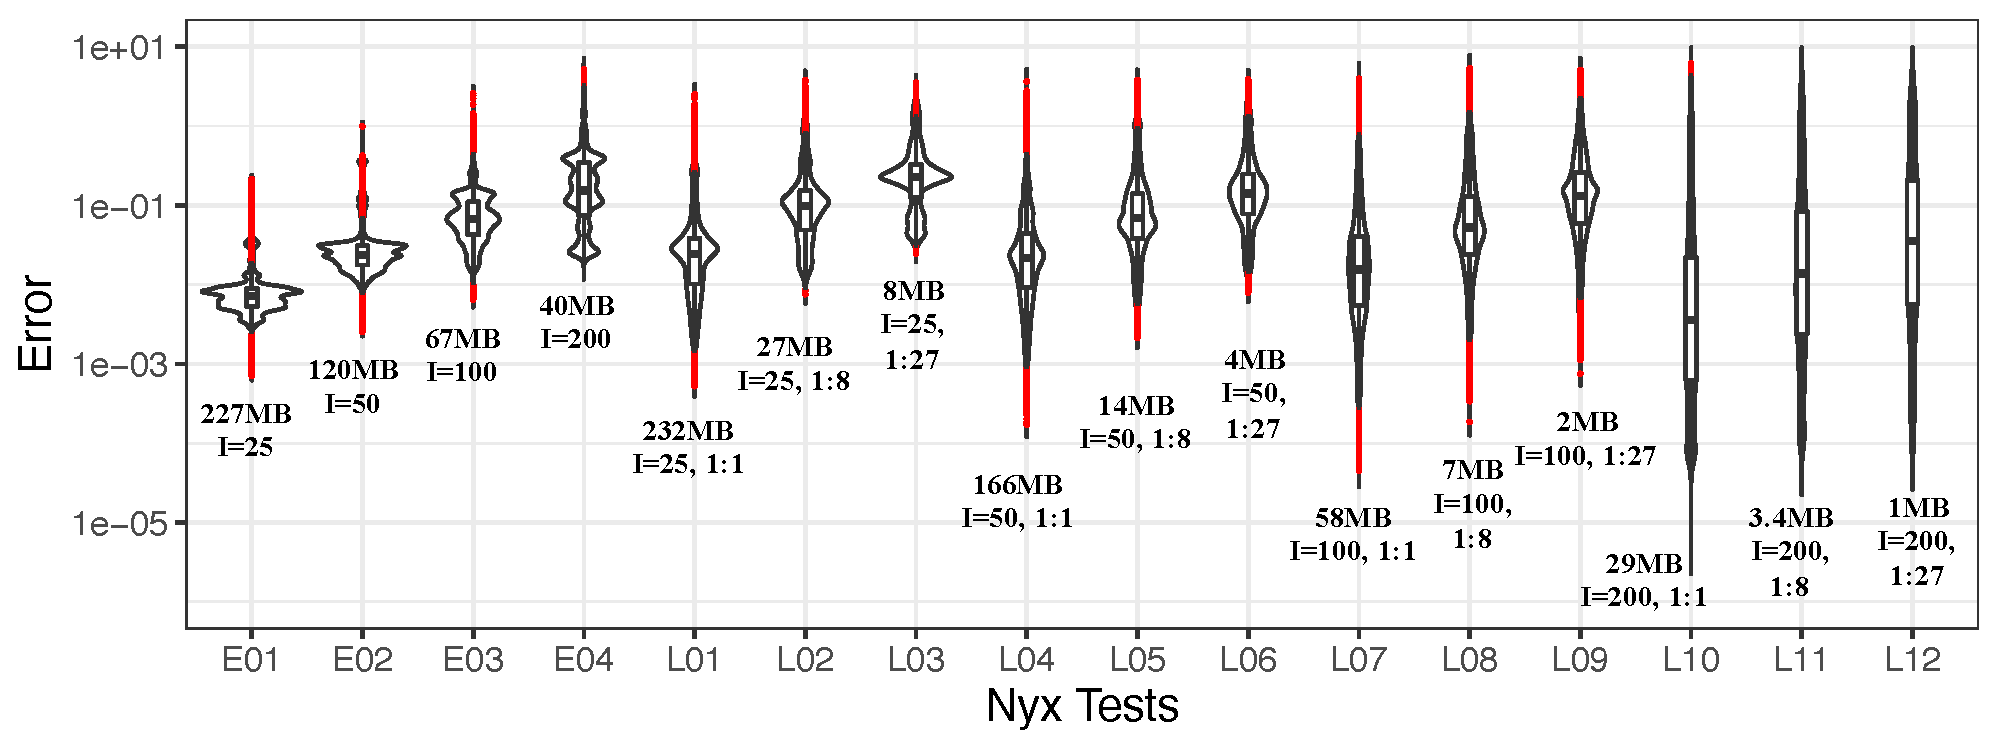
\includegraphics[width=\linewidth]{Images/nyx_violinplot.pdf}
\vspace{-5mm}
\caption{Efficacy results for the Nyx experiments. Each violin plot shows the distribution of the particle reconstruction error for a specific configuration and the horizontal blue dashed line in the chart represents an error equivalent to a single grid cell side. While Eulerian configurations contain greater uncertainty as the value of storage interval \textbf{I} increases, the Lagrangian representations offer the opportunity for improvements in accuracy. Additionally, we find high reconstruction accuracy relies on a high spatial sampling resolution as well.}
\label{fig:nyx_violinplot}
\end{figure}

\begin{figure}[!t]
\centering
\includegraphics[width=\linewidth]{Images/nyx_figure.pdf}
\vspace{-5mm}
\caption{Pathline visualization of baryonic particles evolution in self-gravitating gas dynamics of Nyx simulation. Using 10,000 randomly seeded particles, we visualize pathlines over 300 cycles. To focus on regions where particles cluster to form dense regions, we set opacity of the pathline to be directly proportional to time. Thus, we are able to focus on clustering as well as provide context of transport toward these regions. Lagrangian representations are able to reconstruct the ground truth trajectories and capture clustering accurately when a high spatial sampling is used~(1:1, 1:8). However, when using a 1:27 data reduction factor, some clusters are visualized less clearly.} 
\vspace{-5mm}
\label{fig:nyx_figure}
\end{figure}


\noindent\textbf{Post Hoc Efficacy}
To evaluate the usefulness of Lagrangian representations to encode time-varying self-gravitating gas dynamics, we considered three options for data reduction (1:1, 1:8, 1:27) and four options for \textbf{I}~(25, 50, 100, 200).
%
We constructed pathlines for 50,000 randomly placed particles over 400 cycles during post hoc analysis.
%
%We measure the error of reconstruction of each pathline by comparing to ground truth trajectories.
%
%Additionally, we compute pathlines using Eulerian representations at full spatial resolution and same options for \textbf{I}.
%
We visualize the distribution of reconstruction error for all tests in Figure~\ref{fig:nyx_violinplot}.
%We measure the error or reconstruction of each pathline. and visualize the distribution in Figure~\ref{} along with  
%

The self-gravitating gas dynamics of this simulation produce a vector field that captures the transport of randomly distributed particles to multiple high-density clusters.
%
Particles travel with increasing velocity as clusters increase in density.
%
For this data, we found that Eulerian temporal subsampling performs better for small values of \textbf{I}.
%
This result can be expected given reconstruction using an Eulerian representation and fourth-order Runge Kutta interpolation remain more accurate than second-order barycentric coordinates interpolation employed to interpolate Lagrangian representations~\cite{bujack2015lagrangian}\cite{hummel2016error}.
%
%This can be expected for two reasons: 1) for small values of \textbf{I}, trajectories computed using fourth-order RK4 and Eulerian representations can remain more accurate than second-order barycentric coordinates interpolation and Lagrangian representations (although these are computed in situ using fourth-order RK4), and 2) use of several short Lagrangian flow maps can result in a higher error propagation and accumulation~\cite{bujack2015lagrangian,hummel2016error}.
%
However, as the value of \textbf{I} increases, the distribution of error for the Lagrangian tests indicates that a larger percentage of samples are reconstructed more accurately.
%
The Lagrangian representation computed in situ using RK4 encodes the behavior over an interval of time more accurately for the majority of samples.
%
In contrast, Eulerian representations become less effective at reconstructing the vector field due to increased numerical approximation and accumulating error.
%
%With regard to spatial sampling resolution, for the grid size we consider, we find that reducing the number of samples has a considerable impact on the efficacy of reconstruction.
%
%This indicates that small changes in starting location can result in particles transporting to different clusters.
%

We used pathlines with manually set transfer functions to visualize the evolution and clustering of particles in regions of high density.
%
The total size of the simulation vector field data used to compute the ground truth is 5.3GB.
%
We visualize a random subset of 10,000 pathlines in Figure~\ref{fig:nyx_figure} for configurations with \textbf{I} set to 25.
%To visualize the evolution and clustering of particles in regions of high density, we visualize a random subset of 10,000 pathlines in Figure~\ref{fig:nyx_figure} for configurations with \textbf{I} set to 25.
%
We note that Lagrangian configurations (L04 to L12) using larger values of \textbf{I} are more accurate statistically~(Figure~\ref{fig:nyx_violinplot}).
%
%
The Lagrangian representations demonstrate the ability to closely reconstruct regions where dense clusters are formed while requiring a fraction of the total simulation data size.
%
For example, the 1:8 Lagrangian configuration enables the visualization of transport to dense clusters while requiring only 27MB, i.e., a 200X data reduction of the uncompressed vector field.
%

\vspace{-1mm}
\subsection{SW4 Seismology Simulation}
\label{sec:sw4}
\noindent\textbf{In Situ Encumbrance}
For the SW4 simulation, we considered five grid sizes at varying concurrencies.
%
In each case, we used all six GPUs available on a compute node to execute the simulation and L-ISR.
%
For all L-ISR workloads tested, the execution time required per cycle remained under 0.5 seconds on average, and the maximum in situ memory required by a node was 112 MB to compute the trajectories for 4.4M particles.
%
The cost for performing L-ISR was most dependent on the number of particles and only slightly impacted by increasing grid sizes.
%
%Figure~\ref{fig:insitucost} provides insight regarding performance using GPUs and CPUs. 
%
Referencing Figure~\ref{fig:insitucost}, although the SW4 experiments used six GPUs, we found execution time to be slower than Nyx experiments due to the use of shared memory by multiple ranks~(each has its own data block) and the high cost of launching kernels on the GPU for limited amounts of computation~(each basis particle advances by only a single step/cycle each invocation). 
%
%Increasing grid sizes, however, typically result in longer \textbf{Sim$_{cycle}$} times, and thus, lower \textbf{DAV\%}.
%
%
%DAV\% was closely related to both the Sim$_{cycle}$ and \textbf{Step} cost.
%
%Using fixed concurrency, fixed data reduction factor, and varying grid sizes, we observed \textbf{DAV\%} decrease from 11.67\% to 4.365\% as the grid size increased.
%
%Using fixed concurrency, fixed grid size, and varying data reduction factor, we observed \textbf{DAV\%} increase from 1.201\% to 6.175\% as the number of particles increased.
%
\begingroup
\setlength{\tabcolsep}{-2pt}
%\renewcommand{\arraystretch}{1} % Default value: 1
\begin{table*}[!b]
%\centering
\begin{tabular}{|P{1.1cm}|P{1.1cm}|P{2.7cm}|P{1.3cm}|P{1.5cm}|P{1.9cm}|P{1.7cm}|P{1.7cm}|}
\hline
Nodes & Ranks & Dimensions & \textbf{Sim$_{cycle}$} & Particles & \textbf{InSituMem} & \textbf{Step} & \textbf{DAV\%} \\ 
% & Ranks & & & /Node & /Node (MB) & & \\ 
\hline
%\multicolumn{9}{l}{} & \\
%\multicolumn{9}{l}{\textbf{          Cloverleaf3D Proxy Hydrodynamics Application }} \\ %& \multirow{13}{*}{\includegraphics[width=0.93\linewidth]{images/GPU_Step.pdf}}\\
%\cline{1-9}
%\multirow{9}{*}{16} & \multirow{9}{*}{96} & \multirow{9}{*}{$586\times586\times586$} & 20 & 4.73 & \multirow{3}{*}{1.5M} & \multirow{3}{*}{40.2 } & 0.4475 & 9.408 \\
%\cline{4-4}
%& & & 40 & 4.08 & & & 0.3221 & 7.894 \\
%\cline{4-4}
%& & & 60 & 4.39 & & & 0.3838 & 8.742 \\
%\cline{4-6}%\cline{6-6}
%& & & 20 & 4.50 & \multirow{3}{*}{474k} & \multirow{3}{*}{12 } & 0.1882 & 4.182 \\
%\cline{4-4}
%& & & 40 & 4.14 & & & 0.1628 & 3.932 \\
%\cline{4-4}
%& & & 60 & 4.33 & & & 0.1498 & 3.459 \\
%\cline{4-6}%\cline{6-6}
%& & & 20 & 4.19 & \multirow{3}{*}{186k} & \multirow{3}{*}{4.2 } & 0.0925 & 2.207 \\
%\cline{4-4}
%& & & 40 & 4.11 & & & 0.1043 & 2.537 \\
%\cline{4-4}
%& & & 60 & 3.87 & & & 0.0830 & 2.144 \\
%\cline{1-9}
%%\multicolumn{9}{l}{} & \\
%%\multicolumn{8}{l}{\textbf{          SW4 Seismic Modeling Simulation }}\\
\cline{1-8}
\multirow{3}{*}{1} & \multirow{3}{*}{6} & $251\times251\times70$ & 0.35s & 555k & 13.89MB & 0.0412s & 11.67\% \\
%\cline{3-3}\cline{5-6}
& & $335\times335\times93$  & 2.02s & 1.3M & 33.16MB & 0.2125s & 10.48\% \\
%\cline{3-3}\cline{5-6}  
& & $501\times501\times139$  & 7.58s & 4.4M & 111.13MB & 0.3309s & 4.365\% \\ %& \multirow{13}{*}{\includegraphics[width=0.93\linewidth]{images/CPU_Step.pdf}}\\
\cline{1-3}%\cline{5-6}
\multirow{4}{*}{64} & \multirow{4}{*}{384} & \multirow{3}{*}{$1001\times1001\times276$} & 1.6s & 66k & 1.6MB & 0.0194s & 1.201\% \\
%\cline{6-6}
& & & 1.5s & 146k & 3.6MB & 0.0295s & 1.944\% \\
%\cline{6-6}
& & & 1.3s & 540k & 13.5MB & 0.0798s & 6.175\% \\
\cline{3-3}%\cline{5-6}
& & $1335\times1335\times368$ & 2.9s & 1.2M & 31.9MB & 0.2095s & 7.074\% \\
\cline{1-8}
%\multicolumn{9}{l}{} \\
%\multicolumn{8}{l}{\textbf{          Nyx Cosmology Simulation }} \\
%\cline{1-8}
%\multirow{6}{*}{1} & \multirow{6}{*}{1} & \multirow{3}{*}{$65\times65\times65$} & \multirow{3}{*}{10.9s} & 9k & 0.2MB & 0.0025s & 0.023\% \\
%%\cline{6-6}
%& & & & 32k & 0.8MB & 0.0033s & 0.030\% \\
%%\cline{6-6}
%& & & & 274k & 6.8MB & 0.0122s & 0.0112\% \\
%\cline{3-3}%\cline{5-6}
%& & \multirow{3}{*}{$129\times129\times129$} & \multirow{3}{*}{88.3s} & 32k & 0.8MB & 0.0044s & 0.005\% \\
%%\cline{6-6}
%& & & & 262k & 6.5MB & 0.0101s & 0.011\% \\
%%\cline{6-6}
%& & & & 2.1M & 53.6MB & 0.0596s & 0.067\% \\
\hline
\end{tabular}
\caption{In situ encumbrance evaluation and experiment configurations for the SW4 simulation executing on GPUs. Overall, the \textbf{DAV\%} depends on the number of grid points per rank, the number of particles, i.e., the spatial sampling resolution, as well as the \textbf{Sim$_{cycle}$}.}
%We find \textbf{Sim$_{cycle}$} is more sensitive to the grid dimensions than the cost to perform L-ISR. As the grid dimensions increase, the \textbf{Sim$_{cycle}$} increases and thus, \textbf{DAV\%} decreases. For a fixed grid size, the \textbf{DAV\%} is directly proportional to the spatial sampling resolution, i.e., the number of particles.}
\label{table:sw4_encumbrance}
\end{table*}
\endgroup


\begin{figure}[!b]
\vspace{-5mm}
\begin{subfigure}{0.495\textwidth}
\centering
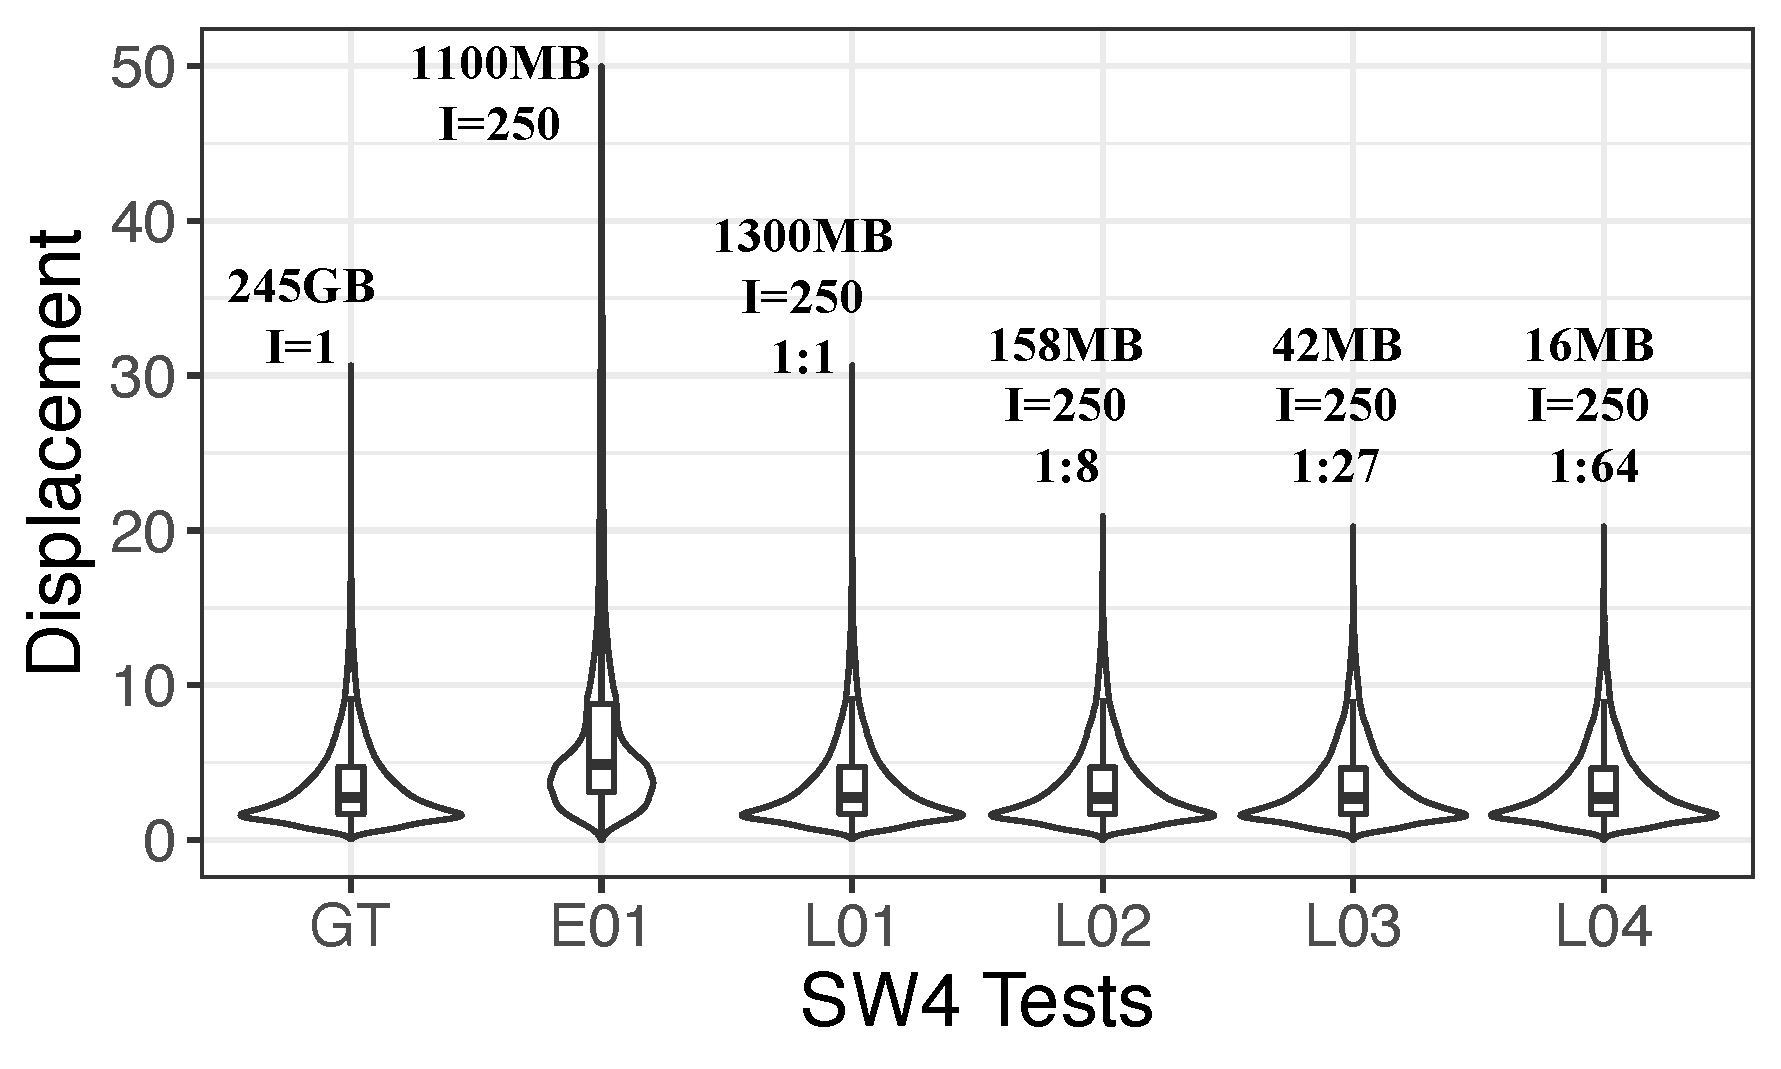
\includegraphics[width=\linewidth]{Images/sw4_violinplot1.pdf}
\vspace{-5mm}
\caption{High displacement near the epicenter.}
\label{fig:epicenter}
\end{subfigure}
\begin{subfigure}{0.495\textwidth}
\centering
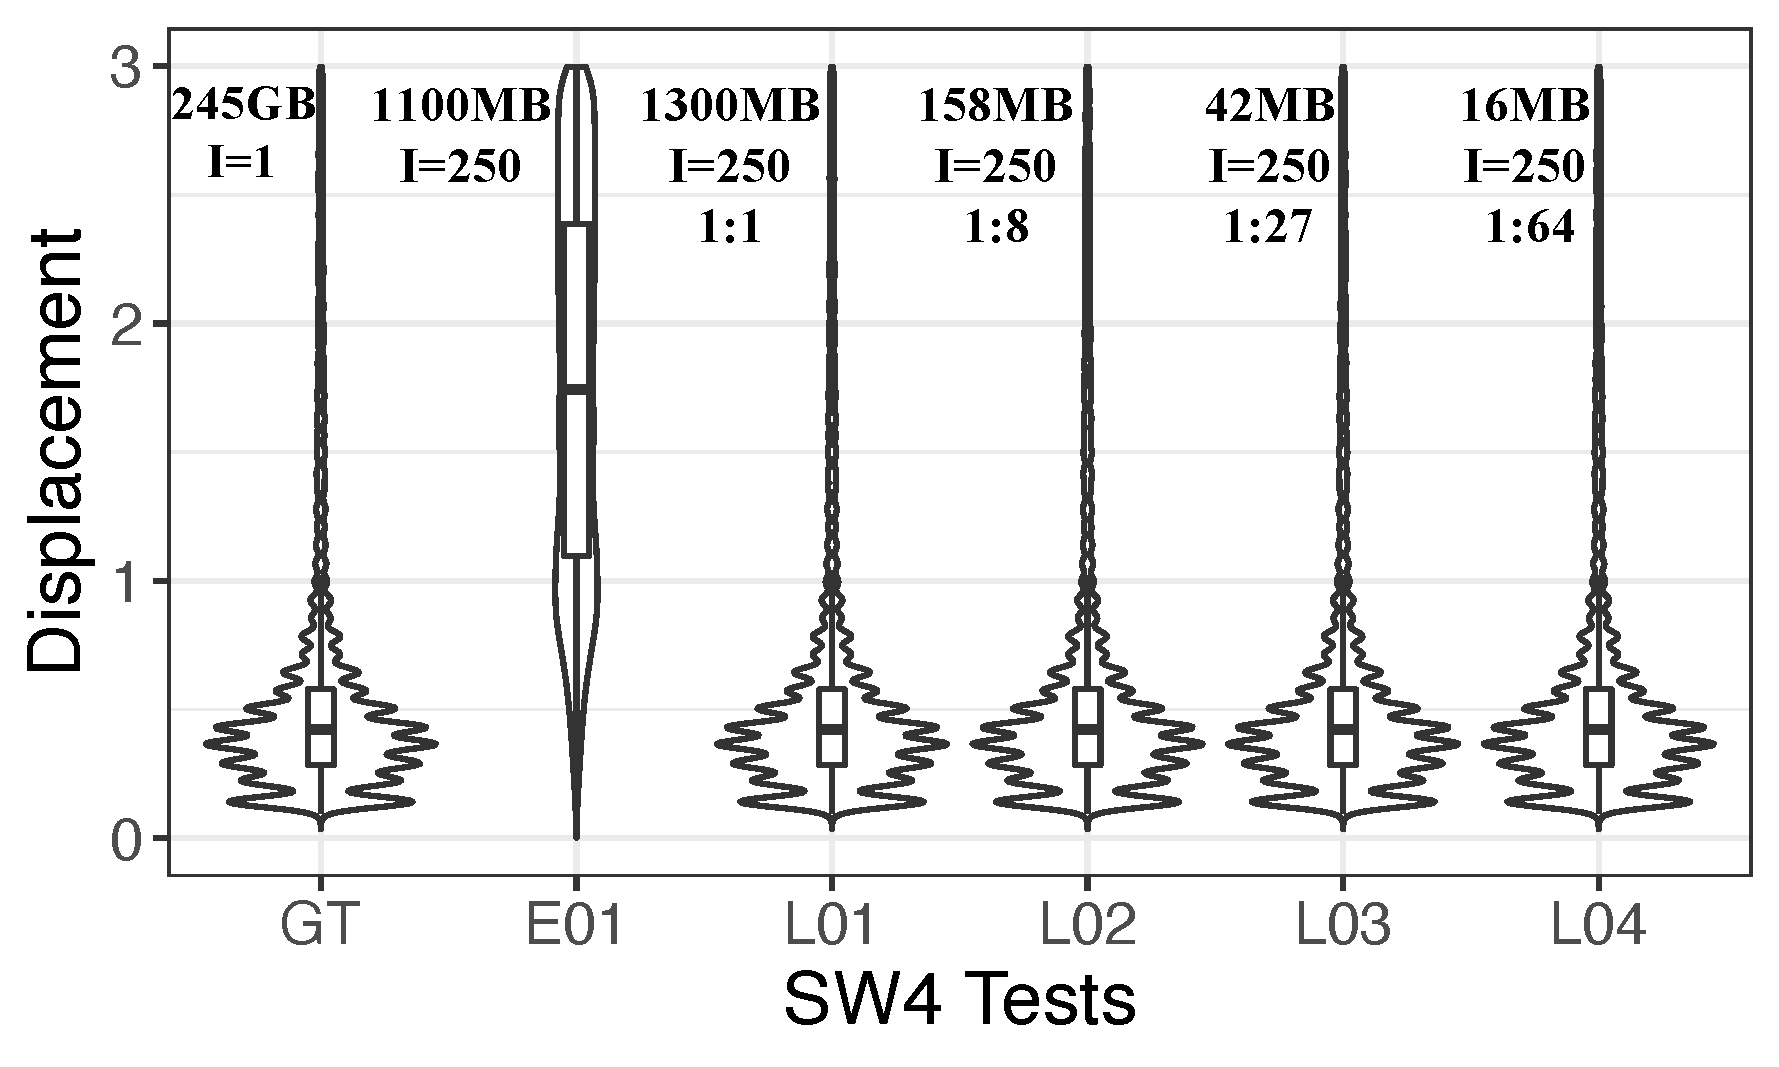
\includegraphics[width=\linewidth]{Images/sw4_violinplot2.pdf}
\vspace{-5mm}
\caption{Low displacement away from the epicenter.}
\label{fig:clusters}
\end{subfigure}
\vspace{-2mm}
\caption{Violin plots of the distribution of particle displacement for the ground truth (GT), one Eulerian configuration and four Lagrangian configurations. The Eulerian configuration, with access to a limited number of time slices, overestimates the displacement. The Lagrangian representation captures displacement in both settings, in regions near and away from the epicenter, accurately.}
\vspace{-5mm}
\label{fig:sw4_violinplot}
\end{figure}

\begin{figure}[!t]
\centering
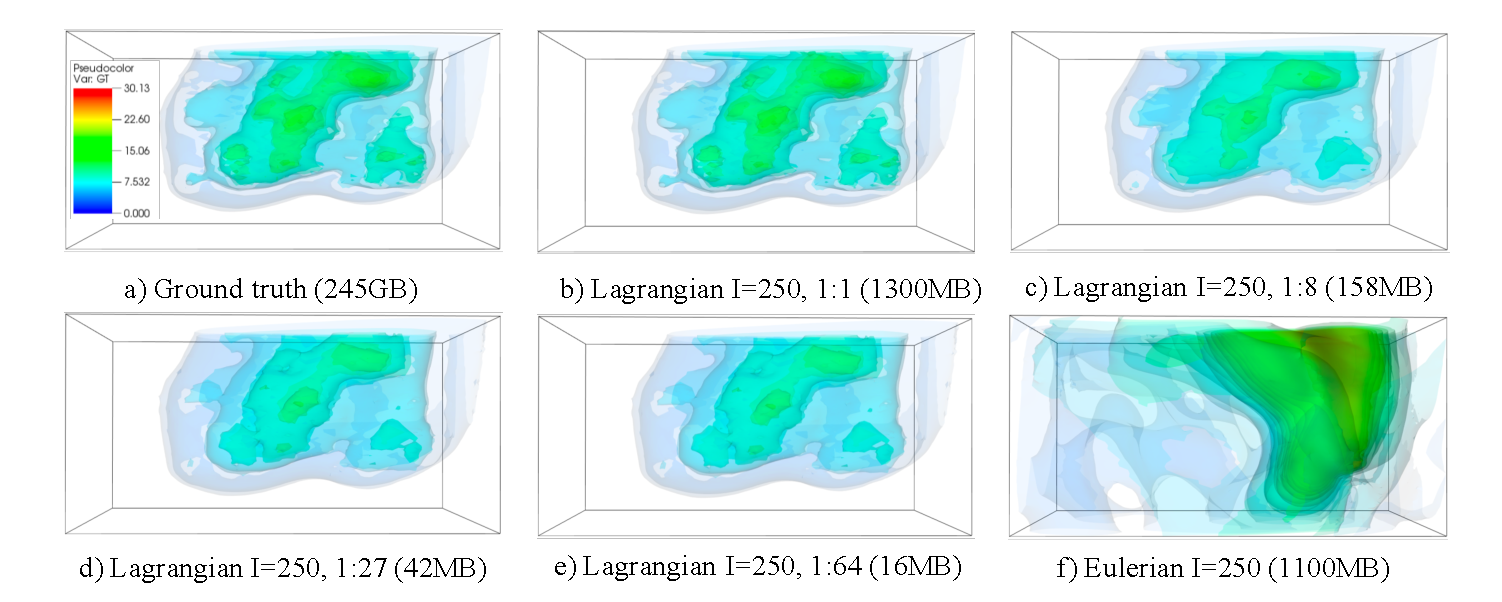
\includegraphics[width=\linewidth, trim={1cm, 0cm, 0.9cm, 0cm}, clip]{Images/sw4_figure_small.pdf}
\vspace{-2mm}
\caption{Visualization of the displacement field derived from reduced Lagrangian representations near the epicenter using multiple isosurfaces. The ground truth is computed using 2000 cycles of the seismic wave propagation simulation. Although at higher data reduction factors regions of high displacement are underestimated, Lagrangian representations are capable of accurately reconstructing the overall feature structure.} 
\vspace{-5mm}
\label{fig:sw4_figure}
\end{figure}


\noindent\textbf{Post Hoc Efficacy}
We studied the reconstruction of the time-varying displacement vector field encoding wave propagation by considering four options for data reduction~(1:1, 1:8, 1:27, 1:64) and 1 option for \textbf{I}~(250).
%
The ground truth was computed using 2000 simulation cycles and required 245 GB.
%
The displacement was highest near the epicenter and reduced as waves propagate further away.
%
For each simulation run, we measured the displacement of 200,000 samples reconstructed near the epicenter (Figure~\ref{fig:epicenter}) and 90,000 samples reconstructed in six regions away from the epicenter (Figure~\ref{fig:clusters}).
%
Here, we directly compare against the distribution of ground truth (GT) displacement.
%
In both cases, Lagrangian representations offered significant data reduction while maintaining high accuracy.
%
We found that as the number of basis trajectories extracted reduces, the displacement for some samples near the epicenter can be underestimated. 
%
In contrast, using a temporally subsampled Eulerian representation (E01) results in significant overestimation of displacement.
%
This result can be expected since temporal subsampling fails to capture the transient nature of wave propagation, whereas Lagrangian representations encoding behavior over an interval of time remain accurate.
%
Compared to Figure~\ref{fig:epicenter}, the ground truth in Figure~\ref{fig:clusters} has smaller displacement and a multimodal distribution that is the result of samples collected from six regions of the domain away from the epicenter. 
%

Figure~\ref{fig:sw4_figure} visualizes the displacement field near the epicenter using multiple semi-opaque isosurfaces.
%
Although the overall structure is well reconstructed using Lagrangian representations, regions of highest displacement can be underestimated as the data reduction factor increases.
%
Overall, we found that Lagrangian representations offer high data reduction options for small loss of accuracy and should be considered more widely for seismic wave propagation vector fields.

%\subsection{Benchmarking Study: Cloverleaf3D}
%\label{sec:cloverleaf3d}



\section{Conclusion}
\label{sec:conclusion}
Accurate exploratory analysis and visualization of time-varying vector fields is challenging.
%
On the one hand, it can be performed accurately if the entire spatiotemporal resolution is available.
%
However, storing all the data to disk for exploratory post hoc analysis is expensive.
%
On the other hand, if subsets of the data are stored, predicting uncertainty and variability of efficacy for analysis techniques post hoc is difficult.
%
In this context, Lagrangian representations computed using the full spatiotemporal resolution via in situ processing demonstrate the potential to enable accurate exploratory time-varying vector field analysis for reduced data storage costs.


%can enable exploratory time-varying vector field analysis.

For wider adoption and consideration of Lagrangian representations, an important step is characterization of effectiveness across a broad range of real-world applications.
%
In this paper, we investigated in situ reduction via Lagrangian representations for vector fields from Nyx cosmology and SW4 seismology simulations.
%
For the Nyx cosmology simulation, we found that Lagrangian representations are sensitive to both the spatial and temporal sampling rate.
%
Notably, providing higher reconstruction accuracy when basis trajectories are computed using a high spatial and low temporal resolution.
%
For the SW4 seismology simulation, we found Lagrangian representations are inherently suited to capture the transient seismic waves and offer high data reduction options for a small loss of accuracy.
%
For both simulations, the percentage of execution time spent on computing the Lagrangian representation in situ was under 10\% in most cases.
%
Overall, we believe the two computational science simulations considered and many others could benefit from Lagrangian representations to enable time-varying vector field exploration. 



%\section{First Section}
%\subsection{A Subsection Sample}
%Please note that the first paragraph of a section or subsection is
%not indented. The first paragraph that follows a table, figure,
%equation etc. does not need an indent, either.
%
%Subsequent paragraphs, however, are indented.
%
%\subsubsection{Sample Heading (Third Level)} Only two levels of
%headings should be numbered. Lower level headings remain unnumbered;
%they are formatted as run-in headings.
%
%\paragraph{Sample Heading (Fourth Level)}
%The contribution should contain no more than four levels of
%headings. Table~\ref{tab1} gives a summary of all heading levels.
%
%\begin{table}
%\caption{Table captions should be placed above the
%tables.}\label{tab1}
%\begin{tabular}{|l|l|l|}
%\hline
%Heading level &  Example & Font size and style\\
%\hline
%Title (centered) &  {\Large\bfseries Lecture Notes} & 14 point, bold\\
%1st-level heading &  {\large\bfseries 1 Introduction} & 12 point, bold\\
%2nd-level heading & {\bfseries 2.1 Printing Area} & 10 point, bold\\
%3rd-level heading & {\bfseries Run-in Heading in Bold.} Text follows & 10 point, bold\\
%4th-level heading & {\itshape Lowest Level Heading.} Text follows & 10 point, italic\\
%\hline
%\end{tabular}
%\end{table}
%
%
%\noindent Displayed equations are centered and set on a separate
%line.
%\begin{equation}
%x + y = z
%\end{equation}
%Please try to avoid rasterized images for line-art diagrams and
%schemas. Whenever possible, use vector graphics instead (see
%Fig.~\ref{fig1}).
%
%\begin{figure}
%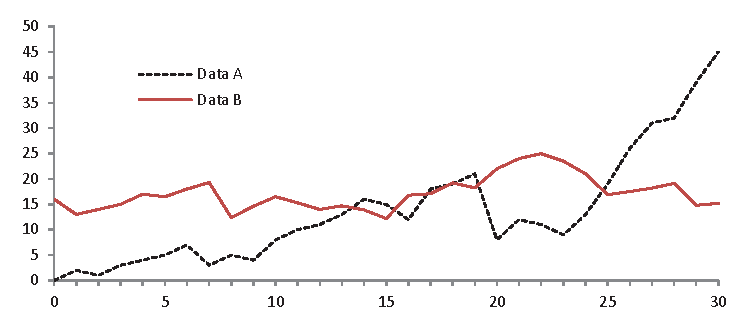
\includegraphics[width=\textwidth]{fig1.eps}
%\caption{A figure caption is always placed below the illustration.
%Please note that short captions are centered, while long ones are
%justified by the macro package automatically.} \label{fig1}
%\end{figure}
%
%\begin{theorem}
%This is a sample theorem. The run-in heading is set in bold, while
%the following text appears in italics. Definitions, lemmas,
%propositions, and corollaries are styled the same way.
%\end{theorem}
%%
%% the environments 'definition', 'lemma', 'proposition', 'corollary',
%% 'remark', and 'example' are defined in the LLNCS documentclass as well.
%%
%\begin{proof}
%Proofs, examples, and remarks have the initial word in italics,
%while the following text appears in normal font.
%\end{proof}
%For citations of references, we prefer the use of square brackets
%and consecutive numbers. Citations using labels or the author/year
%convention are also acceptable. The following bibliography provides
%a sample reference list with entries for journal
%articles~\cite{ref_article1}, an LNCS chapter~\cite{ref_lncs1}, a
%book~\cite{ref_book1}, proceedings without editors~\cite{ref_proc1},
%and a homepage~\cite{ref_url1}. Multiple citations are grouped
%\cite{ref_article1,ref_lncs1,ref_book1},
%\cite{ref_article1,ref_book1,ref_proc1,ref_url1}.
%
% ---- Bibliography ----
%
% BibTeX users should specify bibliography style 'splncs04'.
% References will then be sorted and formatted in the correct style.
%
\bibliographystyle{splncs04}
\bibliography{sane_iccs21}
%
%\begin{thebibliography}{8}
%\bibitem{ref_article1}
%Author, F.: Article title. Journal \textbf{2}(5), 99--110 (2016)
%
%\bibitem{ref_lncs1}
%Author, F., Author, S.: Title of a proceedings paper. In: Editor,
%F., Editor, S. (eds.) CONFERENCE 2016, LNCS, vol. 9999, pp. 1--13.
%Springer, Heidelberg (2016). \doi{10.10007/1234567890}
%
%\bibitem{ref_book1}
%Author, F., Author, S., Author, T.: Book title. 2nd edn. Publisher,
%Location (1999)
%
%\bibitem{ref_proc1}
%Author, A.-B.: Contribution title. In: 9th International Proceedings
%on Proceedings, pp. 1--2. Publisher, Location (2010)
%
%\bibitem{ref_url1}
%LNCS Homepage, \url{http://www.springer.com/lncs}. Last accessed 4
%Oct 2017
%\end{thebibliography}
\end{document}
